\section{Appendix}\label{section:appendix}

%%%%%%%%%%%%%%%%%%%%%%%%%%%%%%%%%%%%%%%%%%%%%%%%%%%%%%%%%%%%%%%%%%%%%%%%%%%%
%%%%%%%%%%%%%%%%%%%%%%%%%%%%%%%%%%%%%%%%%%%%%%%%%%%%%%%%%%%%%%%%%%%%%%%%%%%%
%%%%%%%%%%%%%%%%%%%%%%%%%%%%%%%%%%%%%%%%%%%%%%%%%%%%%%%%%%%%%%%%%%%%%%%%%%%%

\subsection{Pathways}

\begin{figure}[H]
    \centering

    \begin{subfigure}[t]{0.92\linewidth}
        \centering
        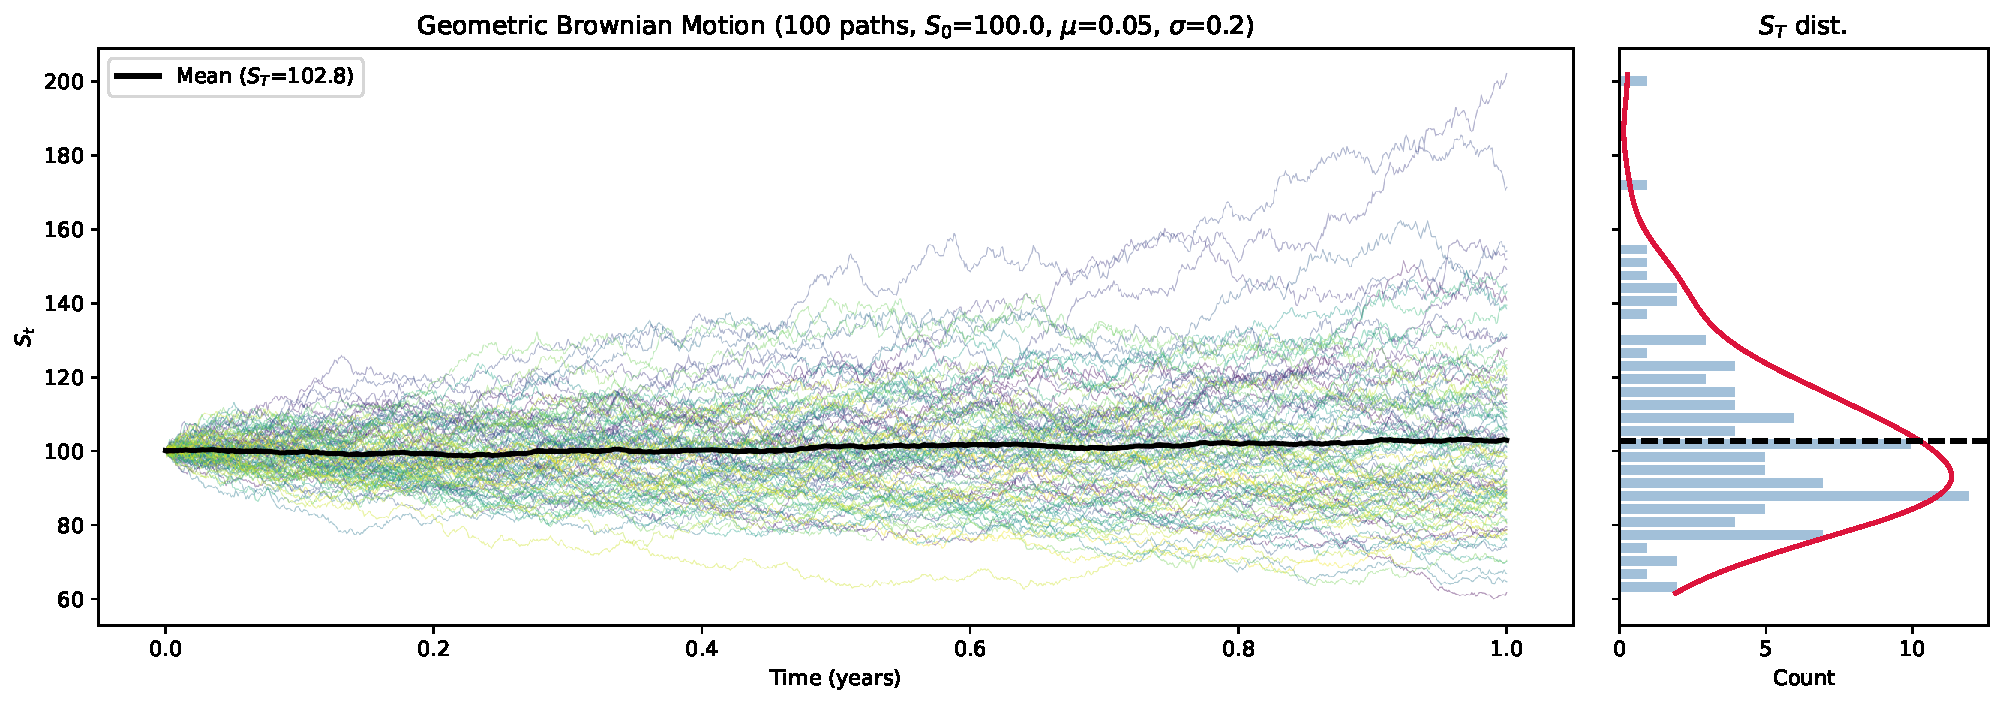
\includegraphics[width=\linewidth]{figures/brownian_path.pdf}
        \caption{Sample Brownian paths used to illustrate the stochastic driving noise in the model setup. The figure provides intuition for the random fluctuations underlying the subsequent Heston dynamics.}
        \label{fig:brownian_path.pdf}
    \end{subfigure}

    \vspace{0.55cm}

    \begin{subfigure}[t]{0.92\linewidth}
        \centering
        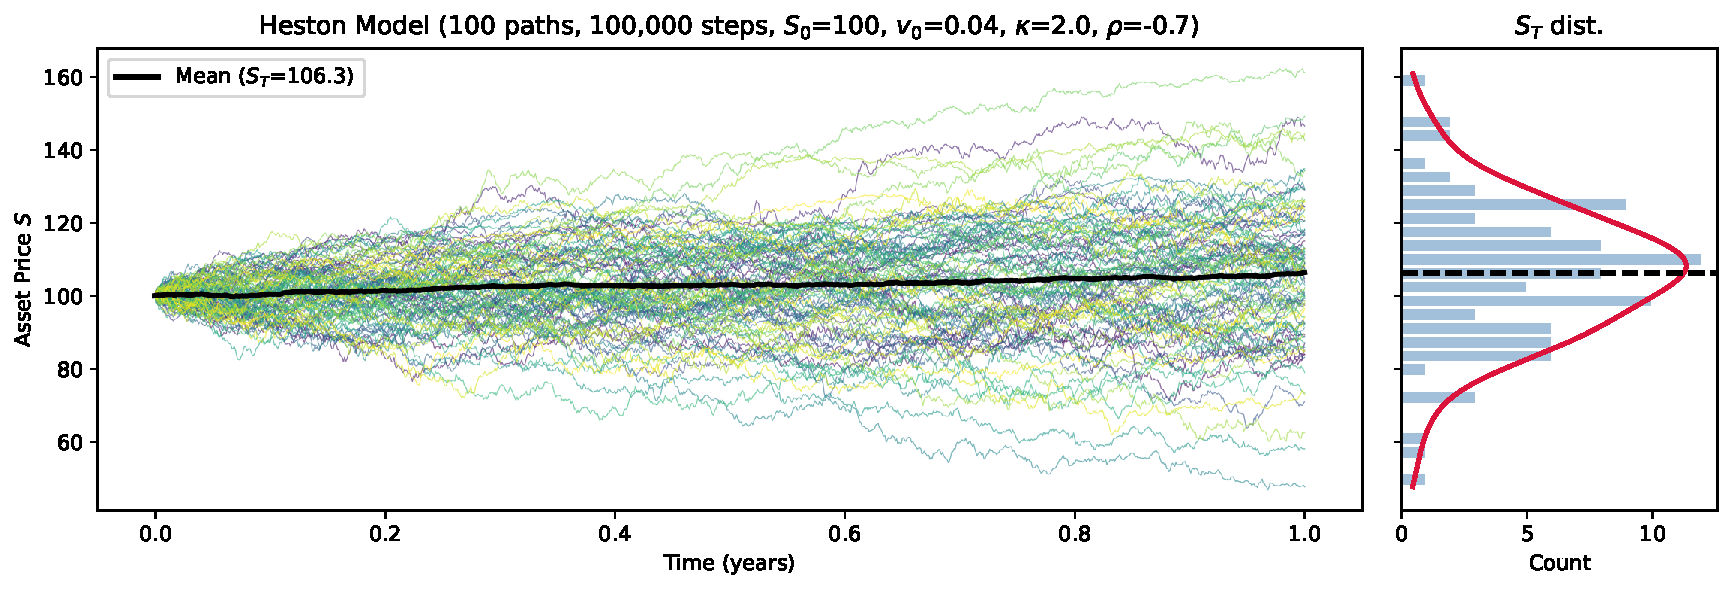
\includegraphics[width=\linewidth]{figures/heston.pdf}
        \caption{Simulated Heston price paths. The figure shows how stochastic volatility generates more realistic and irregular asset-price dynamics than constant-volatility models.}
        \label{fig:heston.pdf}
    \end{subfigure}

    \vspace{0.55cm}

    \begin{subfigure}[t]{0.92\linewidth}
        \centering
        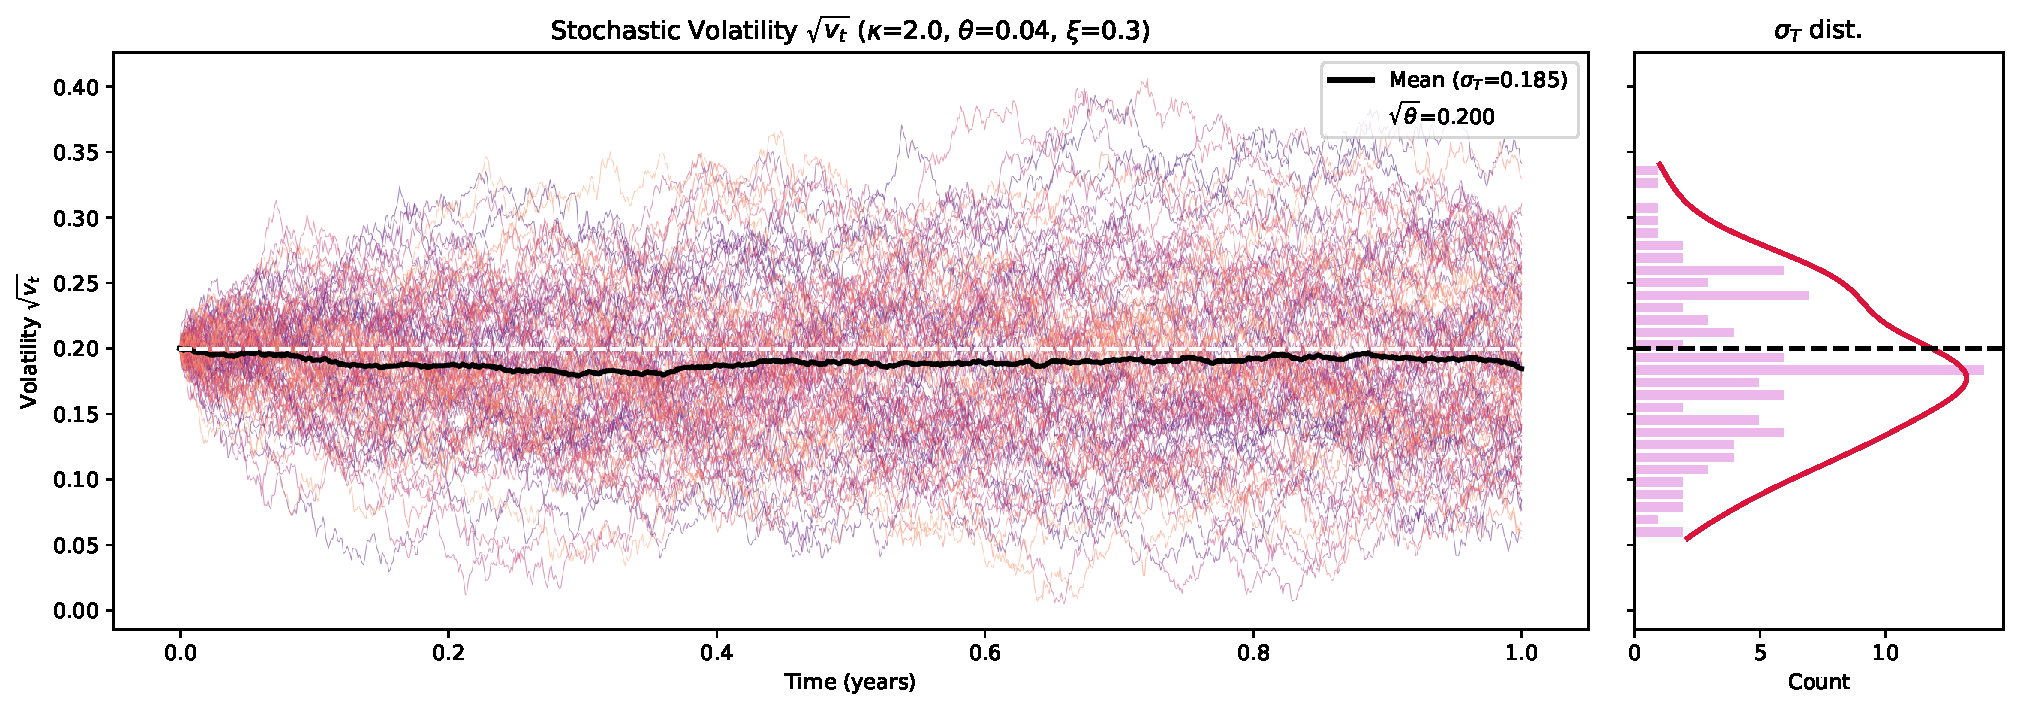
\includegraphics[width=\linewidth]{figures/heston_vol.pdf}
        \caption{Simulated Heston variance or volatility paths. The figure highlights the mean-reverting yet stochastic behavior of volatility in the Heston framework.}
        \label{fig:heston_vol.pdf}
    \end{subfigure}

    \caption{Illustration of the stochastic processes underlying the Heston model. The three panels show Brownian motion, simulated asset-price dynamics, and simulated variance dynamics in a single vertical layout.}
    \label{fig:heston_process_panel}
\end{figure}

%%%%%%%%%%%%%%%%%%%%%%%%%%%%%%%%%%%%%%%%%%%%%%%%%%%%%%%%%%%%%%%%%%%%%%%%%%%%
%%%%%%%%%%%%%%%%%%%%%%%%%%%%%%%%%%%%%%%%%%%%%%%%%%%%%%%%%%%%%%%%%%%%%%%%%%%%
%%%%%%%%%%%%%%%%%%%%%%%%%%%%%%%%%%%%%%%%%%%%%%%%%%%%%%%%%%%%%%%%%%%%%%%%%%%%



\clearpage\subsection{Training duration}

\begin{table}[H]
    \centering
    \begin{minipage}[t]{0.48\linewidth}
        \centering
        \footnotesize
        \setlength{\tabcolsep}{3pt}
        \renewcommand{\arraystretch}{1.2}
        \caption{Black--Scholes PINN training-loss history.}
        \label{tab:bs_training_loss_history}
        \begin{tabular}{rrrrr}
            \hline
            \textbf{Epoch} & \textbf{Total} & \textbf{PDE} & \textbf{IC} & \textbf{BC} \\
            \hline
                 0 & $21994.2520$ & $0.04019$ & $4398.7573$ & $0.01269$ \\
              2500 & $4.31051$    & $0.07313$ & $0.70893$   & $0.00692$ \\
              5000 & $1.17099$    & $0.04505$ & $0.14089$   & $0.00320$ \\
              7500 & $0.83849$    & $0.04067$ & $0.08446$   & $0.00189$ \\
             10000 & $0.77996$    & $0.04238$ & $0.07012$   & $0.00113$ \\
             12500 & $0.63270$    & $0.03394$ & $0.05784$   & $0.00082$ \\
             15000 & $0.44972$    & $0.02157$ & $0.04581$   & $0.00100$ \\
             17500 & $0.44924$    & $0.02296$ & $0.04332$   & $0.00060$ \\
             20000 & $0.41018$    & $0.02141$ & $0.03868$   & $0.00054$ \\
             22500 & $0.31794$    & $0.01427$ & $0.03457$   & $0.00049$ \\
             25000 & $0.26285$    & $0.01070$ & $0.03056$   & $0.00061$ \\
             27500 & $0.21871$    & $0.00805$ & $0.02712$   & $0.00052$ \\
             30000 & $0.19578$    & $0.00702$ & $0.02470$   & $0.00041$ \\
             32500 & $0.17387$    & $0.00561$ & $0.02314$   & $0.00042$ \\
             35000 & $0.15051$    & $0.00394$ & $0.02187$   & $0.00035$ \\
             37500 & $0.13306$    & $0.00286$ & $0.02053$   & $0.00036$ \\
             40000 & $0.13759$    & $0.00390$ & $0.01940$   & $0.00032$ \\
             42500 & $0.11622$    & $0.00228$ & $0.01837$   & $0.00031$ \\
             45000 & $0.11086$    & $0.00220$ & $0.01748$   & $0.00029$ \\
             47500 & $0.10621$    & $0.00212$ & $0.01674$   & $0.00027$ \\
            \hline
        \end{tabular}
    \end{minipage}\hfill
    \begin{minipage}[t]{0.48\linewidth}
        \centering
        \footnotesize
        \setlength{\tabcolsep}{3pt}
        \renewcommand{\arraystretch}{1.2}
        \caption{Heston PINN training-loss history.}
        \label{tab:heston_training_loss_history}
        \begin{tabular}{rrrrr}
            \hline
            \textbf{Epoch} & \textbf{Total} & \textbf{PDE} & \textbf{IC} & \textbf{BC} \\
            \hline
                 0 & $46860.6875$ & $0.03398$  & $4686.0298$ & $0.01044$ \\
              2500 & $137.51643$  & $9.55106$  & $3.99954$   & $0.40209$ \\
              5000 & $125.37741$  & $5.42175$  & $7.08815$   & $0.05568$ \\
              7500 & $58.41161$   & $1.91550$  & $3.91287$   & $0.02558$ \\
             10000 & $202.79363$  & $17.57729$ & $2.69334$   & $0.01747$ \\
             12500 & $266.89291$  & $21.35045$ & $5.33818$   & $0.00133$ \\
             15000 & $50.37729$   & $4.27836$  & $0.75459$   & $0.00957$ \\
             17500 & $47.02234$   & $2.73344$  & $1.95774$   & $0.02211$ \\
             20000 & $35.66247$   & $1.98122$  & $1.57846$   & $0.01313$ \\
             22500 & $18.46533$   & $1.19200$  & $0.65409$   & $0.00090$ \\
             25000 & $10.65871$   & $0.89655$  & $0.16848$   & $0.00168$ \\
             27500 & $7.28630$    & $0.35398$  & $0.37364$   & $0.00202$ \\
             30000 & $5.99006$    & $0.27701$  & $0.32107$   & $0.00186$ \\
             32500 & $2.35999$    & $0.13831$  & $0.09759$   & $0.00020$ \\
             35000 & $1.87818$    & $0.09468$  & $0.09288$   & $0.00052$ \\
             37500 & $1.40915$    & $0.06286$  & $0.07782$   & $0.00047$ \\
             40000 & $1.19361$    & $0.05294$  & $0.06630$   & $0.00024$ \\
             42500 & $0.86779$    & $0.02564$  & $0.06107$   & $0.00015$ \\
             45000 & $0.63638$    & $0.01763$  & $0.04598$   & $0.00007$ \\
             47500 & $0.53413$    & $0.01536$  & $0.03803$   & $0.00005$ \\
            \hline
        \end{tabular}
    \end{minipage}

    \vspace{0.3cm}

    \centering
    \footnotesize
    \setlength{\tabcolsep}{2.5pt}
    \renewcommand{\arraystretch}{1.2}
    \caption{Inverse PINN training and calibration history with evolving parameter estimates $\kappa$, $\theta$, $\xi$, $\rho$.}
    \label{tab:inverse_pinn_calibration_history}
    \begin{adjustbox}{max width=\linewidth}
    \begin{tabular}{rrrrrrrrrrr}
        \hline
        \textbf{Epoch} & \textbf{Total} & \textbf{PDE} & \textbf{IC} & \textbf{BC} & \textbf{Data} & \textbf{Feller} & $\boldsymbol{\kappa}$ & $\boldsymbol{\theta}$ & $\boldsymbol{\xi}$ & $\boldsymbol{\rho}$ \\
        \hline
             0 & $5042358.0000$ & $10.725791$ & $4134.6187$ & $28.860662$ & $5000.6528$ & $0.002455$ & $0.999$ & $0.1001$ & $0.500$ & $-0.001$ \\
          1500 & $4059.0977$    & $87.752625$ & $29.4920$   & $0.367506$  & $2.0073$    & $0.000000$ & $1.620$ & $0.0422$ & $0.163$ & $0.793$ \\
          3000 & $1085.7815$    & $11.841378$ & $7.7701$    & $0.067702$  & $0.7709$    & $0.000000$ & $1.578$ & $0.0357$ & $0.133$ & $0.888$ \\
          4500 & $1028.3889$    & $5.079397$  & $3.6259$    & $0.043186$  & $0.8903$    & $0.000000$ & $1.536$ & $0.0344$ & $0.123$ & $0.921$ \\
          6000 & $283.0856$     & $5.284629$  & $2.4379$    & $0.042856$  & $0.1528$    & $0.000000$ & $1.504$ & $0.0345$ & $0.118$ & $0.940$ \\
          7500 & $1080.6104$    & $21.654047$ & $3.2561$    & $0.109399$  & $0.6144$    & $0.000000$ & $1.485$ & $0.0344$ & $0.115$ & $0.955$ \\
          9000 & $141.1073$     & $2.657735$  & $1.3538$    & $0.017838$  & $0.0743$    & $0.000000$ & $1.484$ & $0.0337$ & $0.112$ & $0.964$ \\
         10500 & $357.5637$     & $5.206030$  & $1.4301$    & $0.059183$  & $0.2388$    & $0.000000$ & $1.469$ & $0.0334$ & $0.110$ & $0.973$ \\
         12000 & $82.9516$      & $1.525354$  & $0.9522$    & $0.021463$  & $0.0428$    & $0.000000$ & $1.480$ & $0.0320$ & $0.109$ & $0.978$ \\
         13500 & $144.8452$     & $3.712763$  & $0.8913$    & $0.042495$  & $0.0615$    & $0.000000$ & $1.493$ & $0.0307$ & $0.107$ & $0.983$ \\
         15000 & $86.0975$      & $1.212989$  & $0.7499$    & $0.004642$  & $0.0543$    & $0.000000$ & $1.501$ & $0.0300$ & $0.107$ & $0.986$ \\
         16500 & $42.8948$      & $1.066067$  & $0.6579$    & $0.002672$  & $0.0150$    & $0.000000$ & $1.514$ & $0.0293$ & $0.107$ & $0.988$ \\
         18000 & $28.8773$      & $0.705716$  & $0.4965$    & $0.002691$  & $0.0098$    & $0.000000$ & $1.536$ & $0.0282$ & $0.106$ & $0.991$ \\
         19500 & $36.3960$      & $1.234485$  & $0.5088$    & $0.004252$  & $0.0066$    & $0.000000$ & $1.548$ & $0.0278$ & $0.106$ & $0.992$ \\
         21000 & $25.2769$      & $0.750561$  & $0.4207$    & $0.003757$  & $0.0060$    & $0.000000$ & $1.562$ & $0.0273$ & $0.105$ & $0.993$ \\
         22500 & $19.7579$      & $0.587920$  & $0.4024$    & $0.002703$  & $0.0040$    & $0.000000$ & $1.574$ & $0.0269$ & $0.105$ & $0.994$ \\
         24000 & $17.8799$      & $0.548446$  & $0.3758$    & $0.002470$  & $0.0031$    & $0.000000$ & $1.584$ & $0.0267$ & $0.105$ & $0.994$ \\
         25500 & $17.3094$      & $0.533012$  & $0.3654$    & $0.002380$  & $0.0030$    & $0.000000$ & $1.588$ & $0.0266$ & $0.104$ & $0.994$ \\
         27000 & $17.3094$      & $0.533012$  & $0.3654$    & $0.002380$  & $0.0030$    & $0.000000$ & $1.588$ & $0.0266$ & $0.104$ & $0.994$ \\
         28500 & $17.3094$      & $0.533012$  & $0.3654$    & $0.002380$  & $0.0030$    & $0.000000$ & $1.588$ & $0.0266$ & $0.104$ & $0.994$ \\
         29999 & $17.3094$      & $0.533012$  & $0.3654$    & $0.002380$  & $0.0030$    & $0.000000$ & $1.588$ & $0.0266$ & $0.104$ & $0.994$ \\
        \hline
    \end{tabular}
    \end{adjustbox}
\end{table}

\vspace{-0.15cm}

\noindent\footnotesize
\textbf{Notes for Tables~\ref{tab:bs_training_loss_history}--\ref{tab:inverse_pinn_calibration_history}.}
\textbf{(BS)} 50000 epochs in 12\,min 8\,s; 6250 points (5000 interior, 1000 IC, 250 BC); final total loss $0.102625$.
\textbf{(Heston)} 50000 epochs in 9\,min 7\,s; 12250 points (10000 interior, 2000 IC, 250 BC); final total loss $0.485010$.
\textbf{(Inverse)} 30000 epochs in 16\,min 27\,s; final losses --- total $17.3094$, PDE $0.533012$, data $0.0030$; final calibrated $\kappa=1.588$, $\theta=0.0266$, $\xi=0.104$, $\rho=0.994$.
\normalsize

%%%%%%%%%%%%%%%%%%%%%%%%%%%%%%%%%%%%%%%%%%%%%%%%%%%%%%%%%%%%%%%%%%%%%%%%%%%%
%%%%%%%%%%%%%%%%%%%%%%%%%%%%%%%%%%%%%%%%%%%%%%%%%%%%%%%%%%%%%%%%%%%%%%%%%%%%
%%%%%%%%%%%%%%%%%%%%%%%%%%%%%%%%%%%%%%%%%%%%%%%%%%%%%%%%%%%%%%%%%%%%%%%%%%%%


\clearpage\subsection{Black-Scholes PINN}

\begin{figure}[H]
    \centering

    \begin{subfigure}[t]{0.49\linewidth}
        \centering
        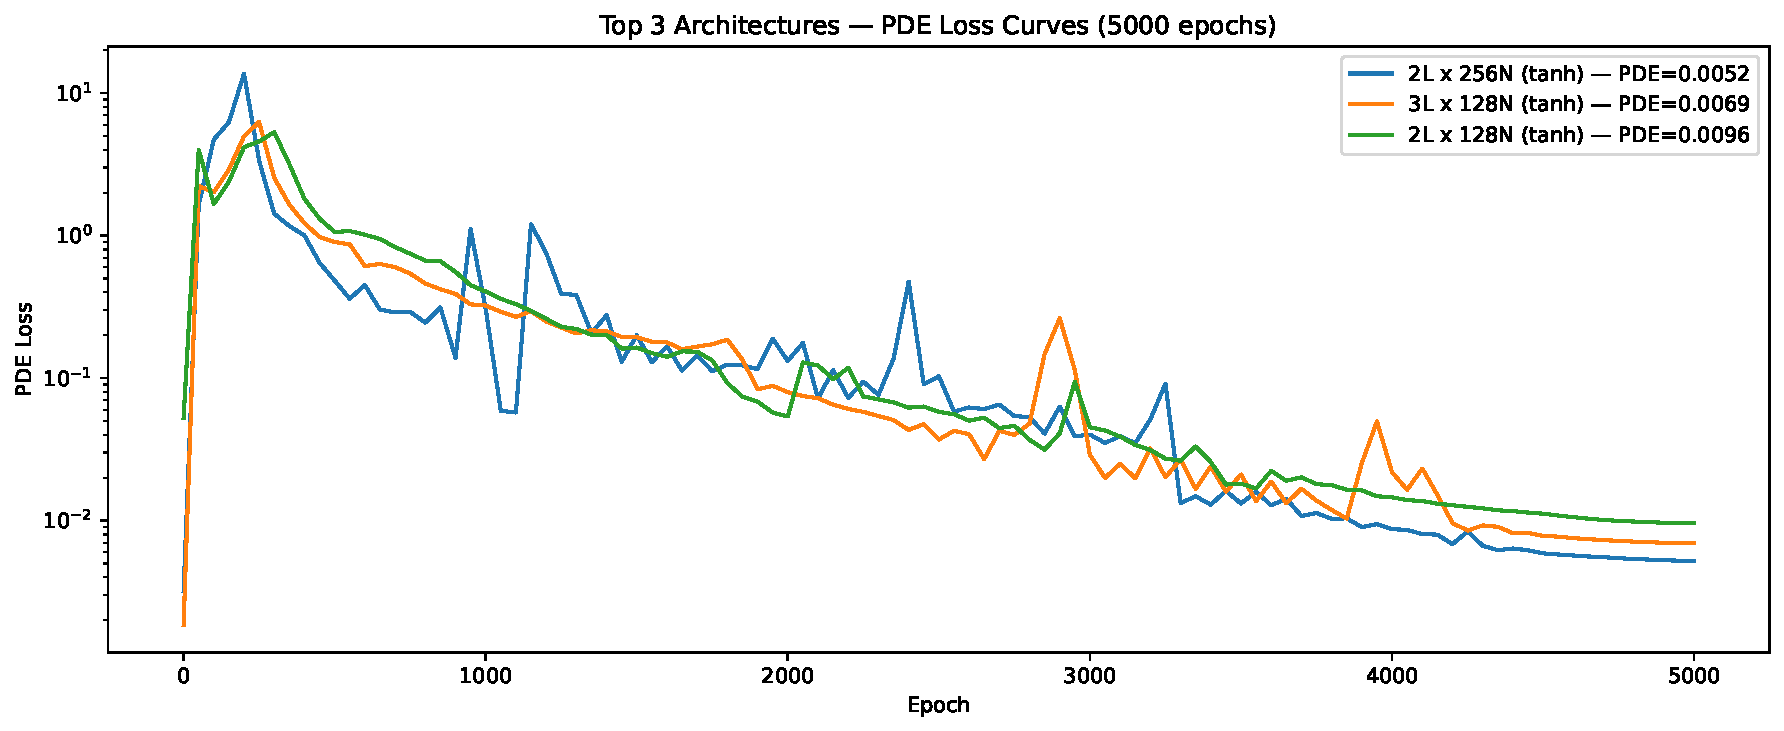
\includegraphics[width=\linewidth]{figures/hyper_bs_arch_top3_curves.pdf}
        \caption{Training curves for the three best-performing Black--Scholes architectures. The plot compares convergence speed and stability, showing whether the leading architectures differ mainly in final accuracy or in optimization dynamics.}
        \label{fig:hyper_bs_arch_top3_curves.pdf}
    \end{subfigure}
    \hfill
    \begin{subfigure}[t]{0.49\linewidth}
        \centering
        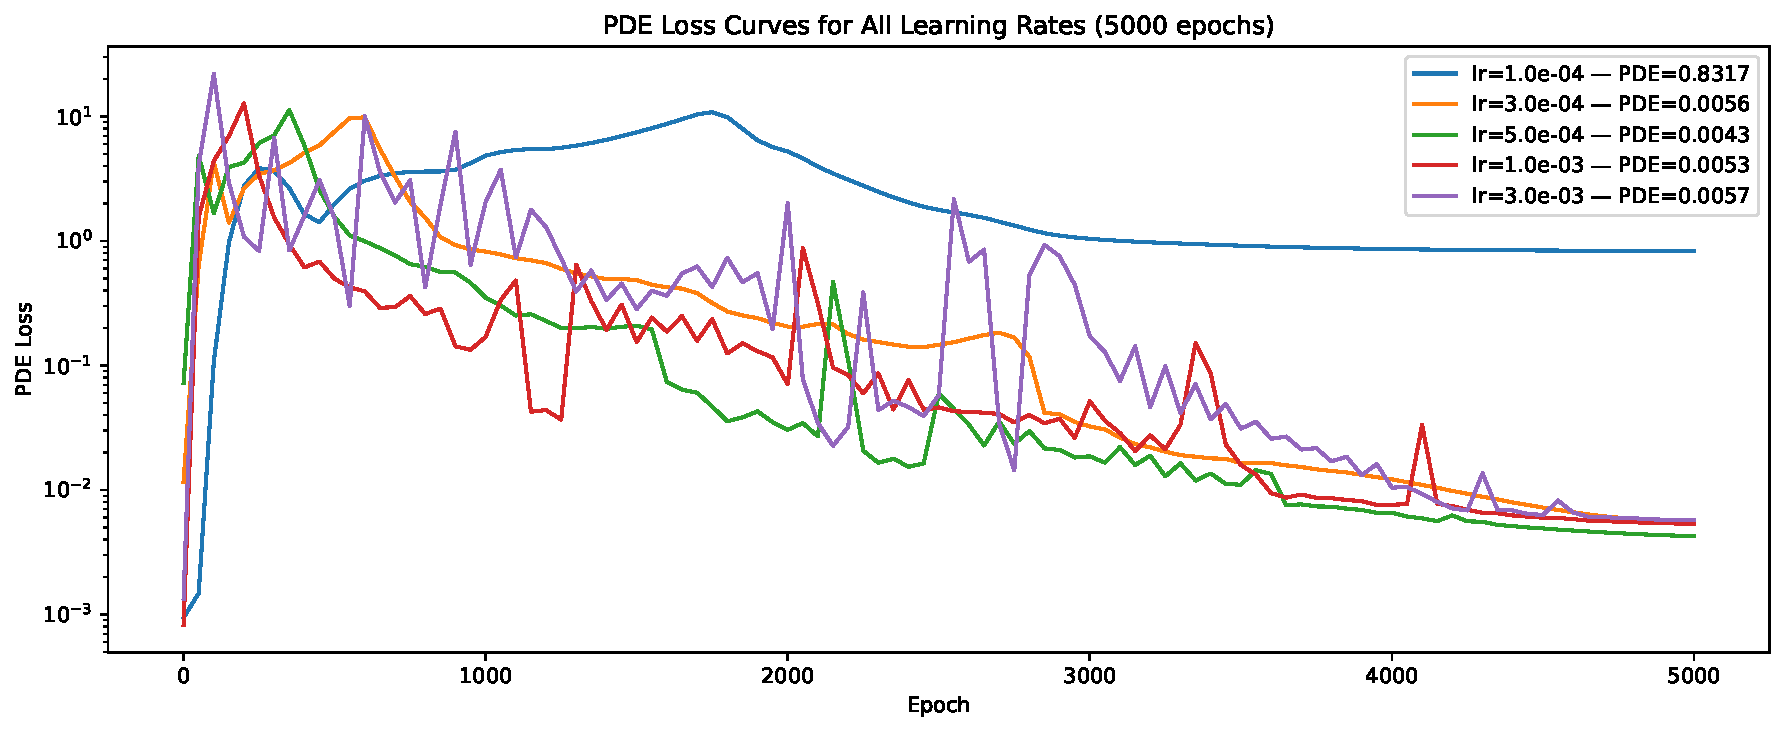
\includegraphics[width=\linewidth]{figures/hyper_bs_lr_curves.pdf}
        \caption{Training curves for the tested Black--Scholes learning rates. The figure shows how learning-rate selection affects convergence speed, oscillation, and the final loss level.}
        \label{fig:hyper_bs_lr_curves.pdf}
    \end{subfigure}

    \vspace{0.5cm}

    \begin{subfigure}[t]{0.49\linewidth}
        \centering
        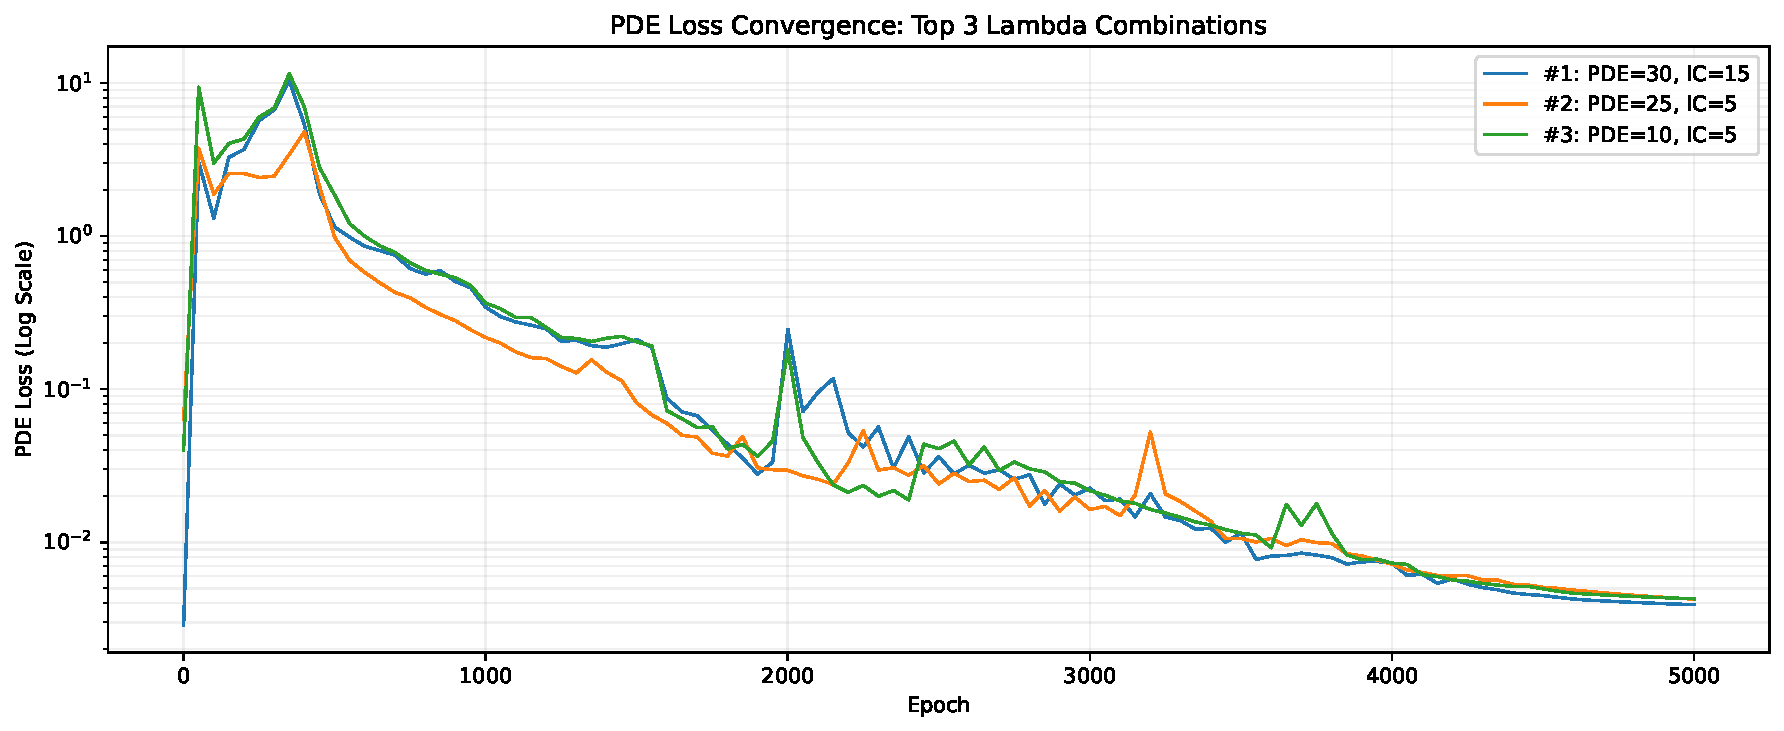
\includegraphics[width=\linewidth]{figures/hyper_bs_top3_curves.pdf}
        \caption{Training curves for the three best-performing Black--Scholes $\lambda$ configurations. The plot shows whether the strongest loss-weight choices produce consistently smooth convergence or only improve final error after longer training.}
        \label{fig:hyper_bs_top3_curves.pdf}
    \end{subfigure}
    \hfill
    \begin{subfigure}[t]{0.49\linewidth}
        \centering
        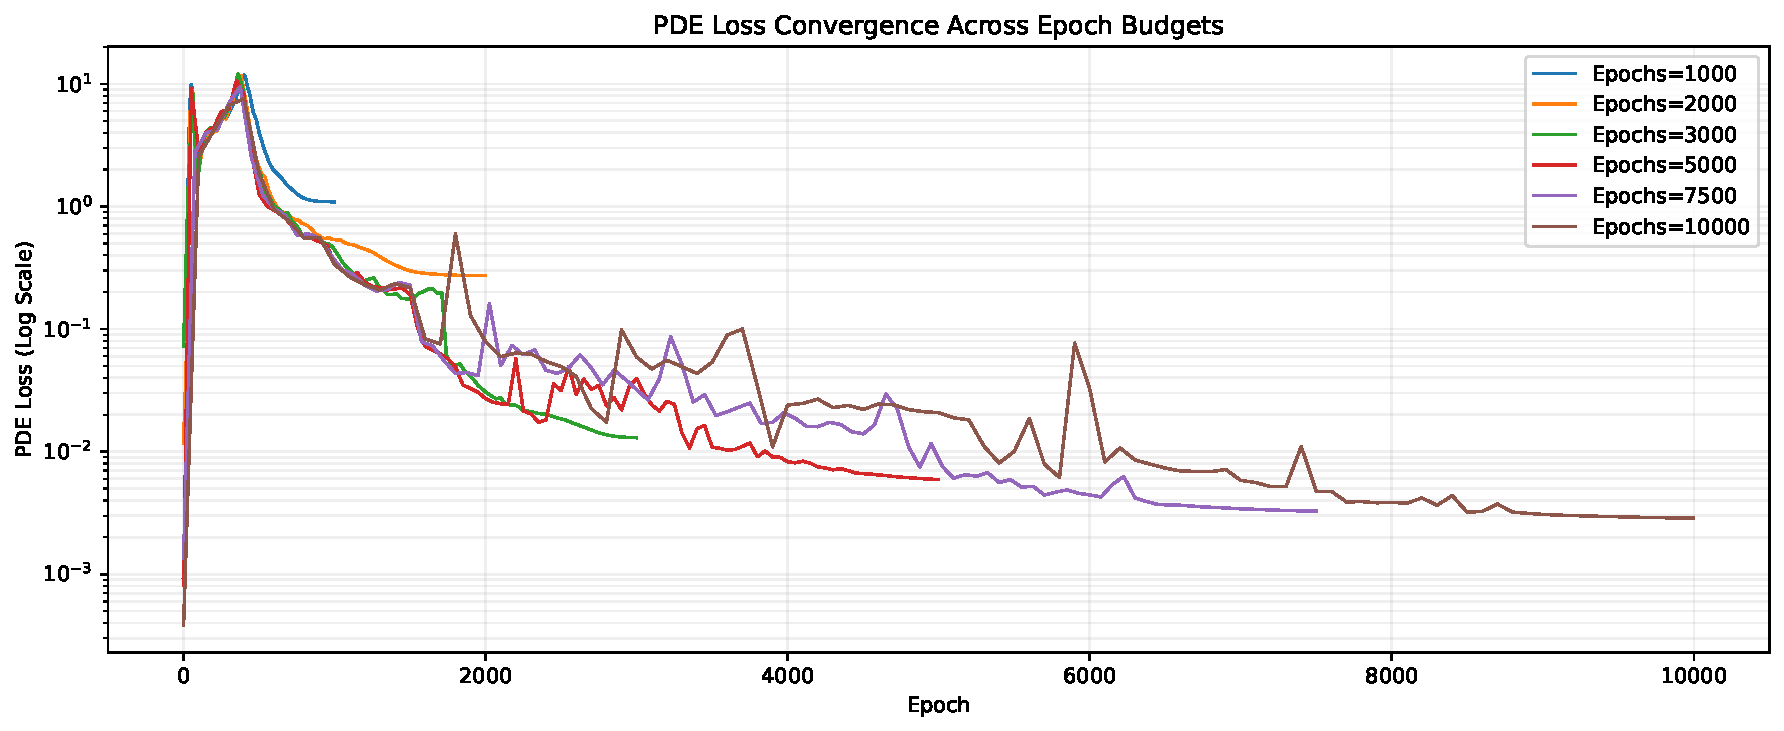
\includegraphics[width=\linewidth]{figures/hyper_bs_conv_curves.pdf}
        \caption{Training curves for the Black--Scholes convergence experiments. The figure illustrates the relationship between training duration, loss decay, and eventual stabilization of the optimization process.}
        \label{fig:hyper_bs_conv_curves.pdf}
    \end{subfigure}

    \caption{Training-curve comparison for the main Black--Scholes hyperparameter experiments. The four panels summarize the effects of architecture choice, learning rate, loss-weight selection, and training duration on convergence behavior.}
    \label{fig:hyper_bs_curves_panel}
\end{figure}

\begin{figure}[H]
    \centering

    \begin{subfigure}[t]{0.49\linewidth}
        \centering
        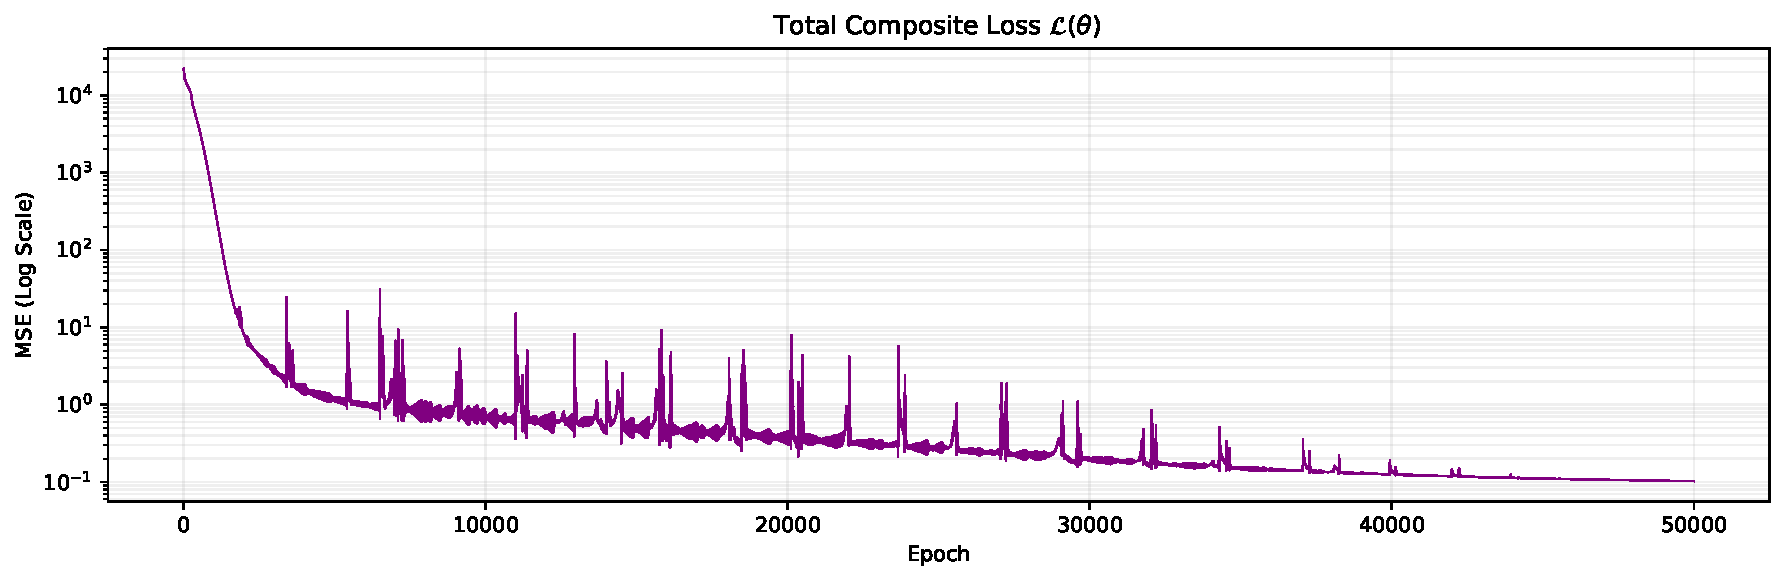
\includegraphics[width=\linewidth]{figures/pinn_bs_loss_total.pdf}
        \caption{Total training loss for the final Black--Scholes PINN. This curve summarizes the overall optimization objective across the full training run.}
        \label{fig:pinn_bs_loss_total.pdf}
    \end{subfigure}
    \hfill
    \begin{subfigure}[t]{0.49\linewidth}
        \centering
        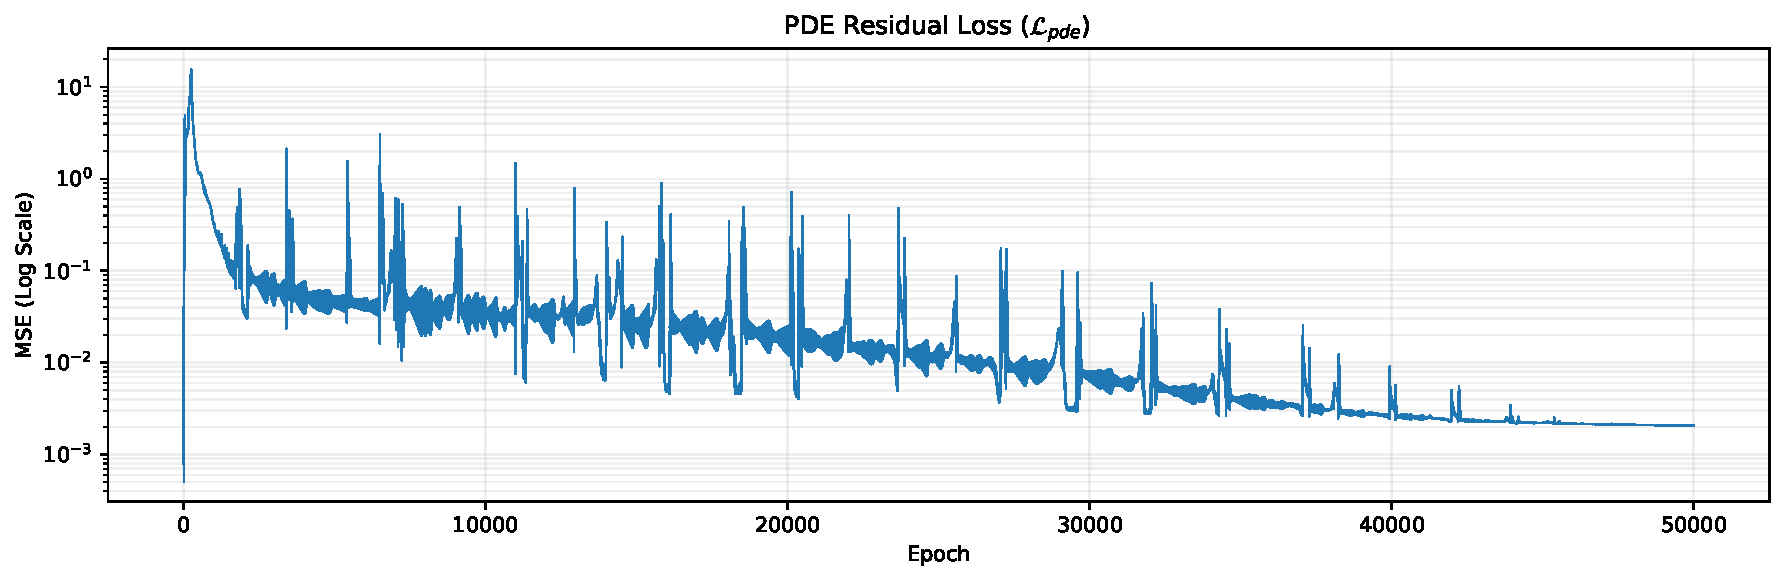
\includegraphics[width=\linewidth]{figures/pinn_bs_loss_pde.pdf}
        \caption{PDE-residual loss for the final Black--Scholes PINN. This component measures how well the learned solution satisfies the Black--Scholes equation in the interior domain.}
        \label{fig:pinn_bs_loss_pde.pdf}
    \end{subfigure}

    \vspace{0.6cm}

    \begin{subfigure}[t]{0.49\linewidth}
        \centering
        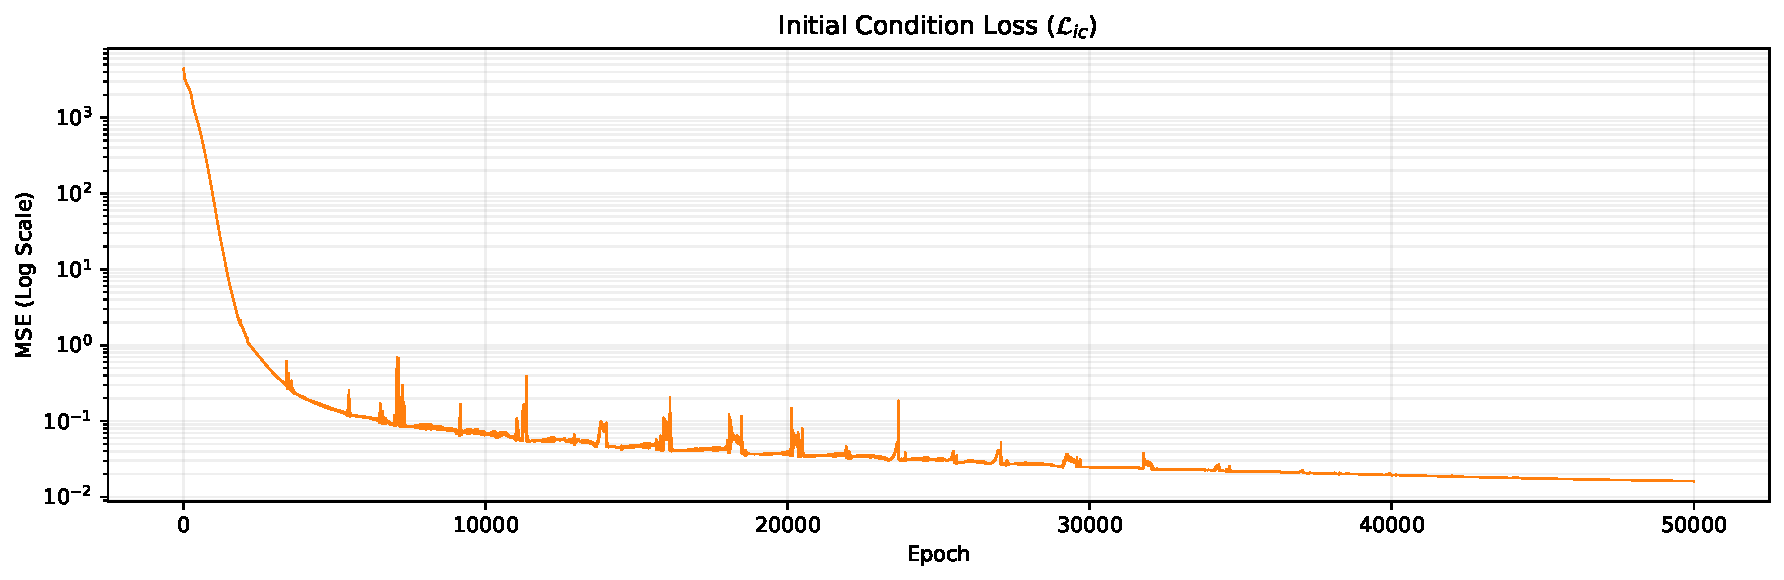
\includegraphics[width=\linewidth]{figures/pinn_bs_loss_ic.pdf}
        \caption{Initial-condition loss for the final Black--Scholes PINN. This term tracks how accurately the payoff condition at maturity is enforced during training.}
        \label{fig:pinn_bs_loss_ic.pdf}
    \end{subfigure}
    \hfill
    \begin{subfigure}[t]{0.49\linewidth}
        \centering
        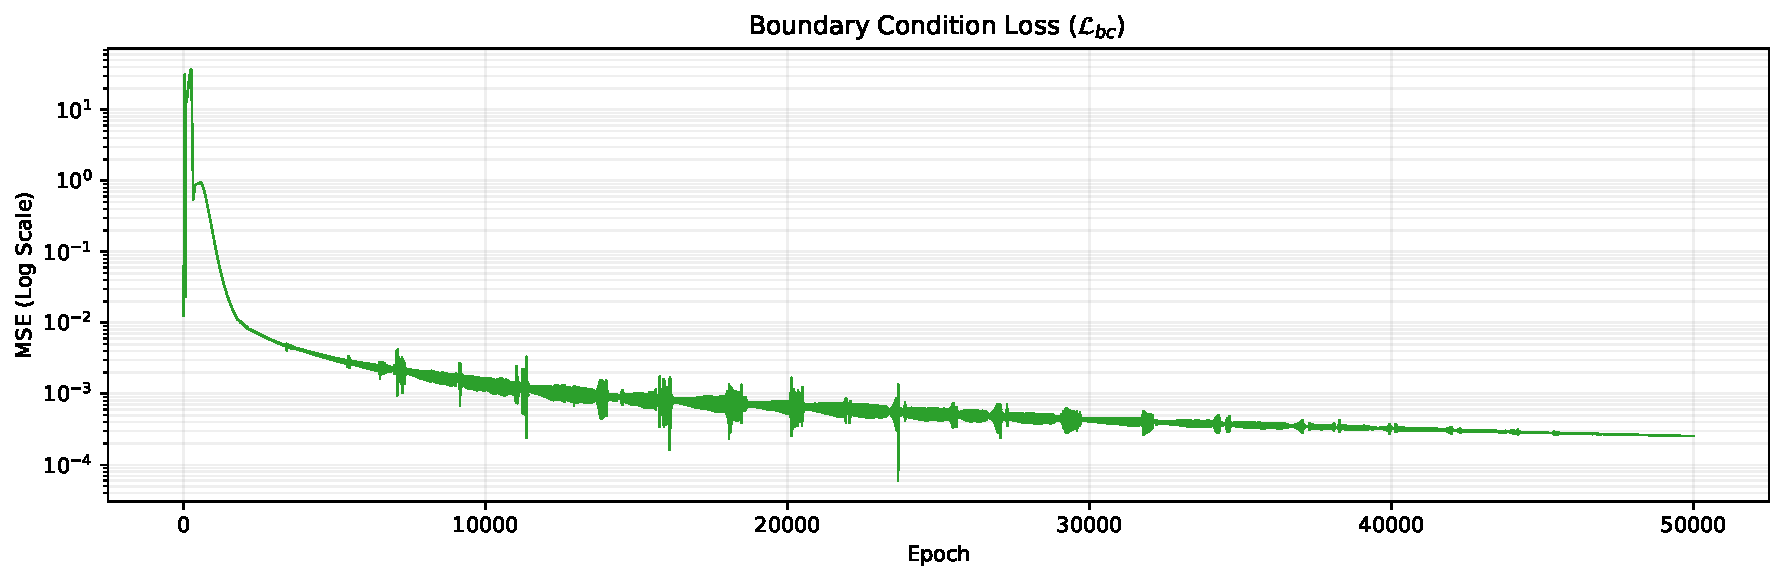
\includegraphics[width=\linewidth]{figures/pinn_bs_loss_bc.pdf}
        \caption{Boundary-condition loss for the final Black--Scholes PINN. This curve shows how well the network respects the imposed boundary behavior at the edges of the spatial domain.}
        \label{fig:pinn_bs_loss_bc.pdf}
    \end{subfigure}

    \caption{Loss decomposition for the final Black--Scholes PINN. The four panels show the evolution of the total, PDE, initial-condition, and boundary-condition losses, providing a compact overview of convergence throughout training.}
    \label{fig:pinn_bs_loss_panel}
\end{figure}

%%%%%%%%%%%%%%%%%%%%%%%%%%%%%%%%%%%%%%%%%%%%%%%%%%%%%%%%%%%%%%%%%%%%%%%%%%%%
%%%%%%%%%%%%%%%%%%%%%%%%%%%%%%%%%%%%%%%%%%%%%%%%%%%%%%%%%%%%%%%%%%%%%%%%%%%%
%%%%%%%%%%%%%%%%%%%%%%%%%%%%%%%%%%%%%%%%%%%%%%%%%%%%%%%%%%%%%%%%%%%%%%%%%%%%

\clearpage\subsection{Heston PINN}

\begin{figure}[H]
    \centering

    \begin{subfigure}[t]{0.49\linewidth}
        \centering
        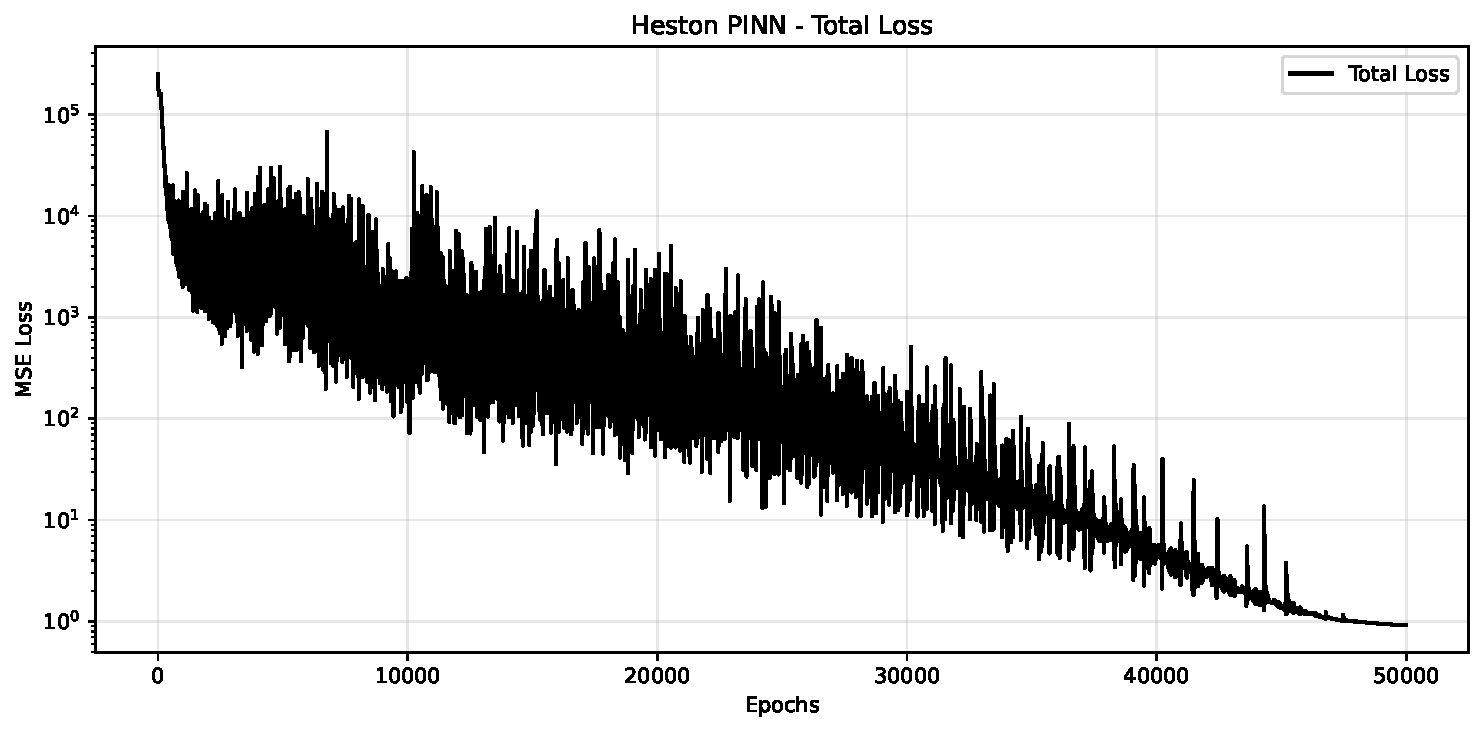
\includegraphics[width=\linewidth]{figures/pinn_hs_loss_total.pdf}
        \caption{Total training loss for the Heston PINN. This curve summarizes the overall optimization objective during training.}
        \label{fig:pinn_hs_loss_total.pdf}
    \end{subfigure}
    \hfill
    \begin{subfigure}[t]{0.49\linewidth}
        \centering
        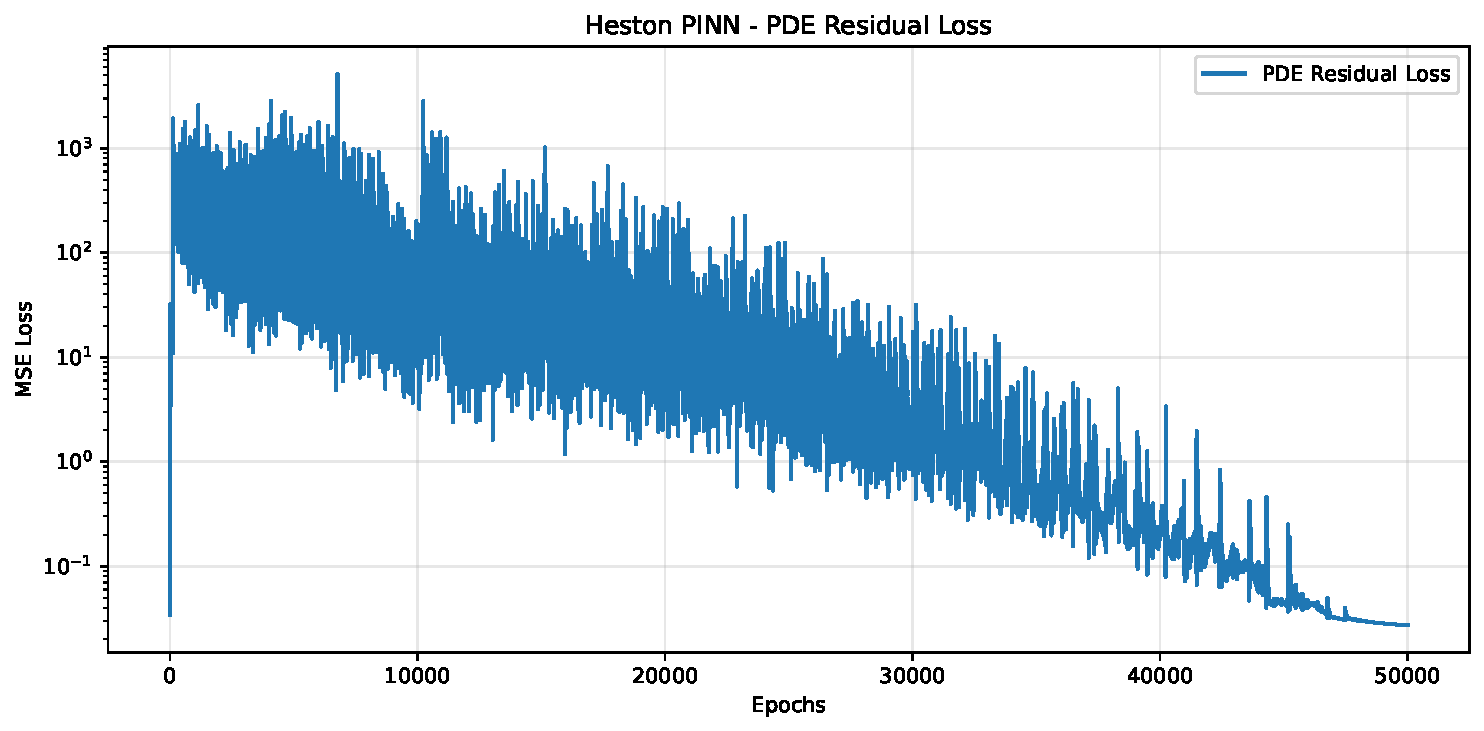
\includegraphics[width=\linewidth]{figures/pinn_hs_loss_pde.pdf}
        \caption{PDE-residual loss for the Heston PINN. This component tracks how well the learned solution satisfies the Heston equation in the interior domain.}
        \label{fig:pinn_hs_loss_pde.pdf}
    \end{subfigure}

    \vspace{0.6cm}

    \begin{subfigure}[t]{0.49\linewidth}
        \centering
        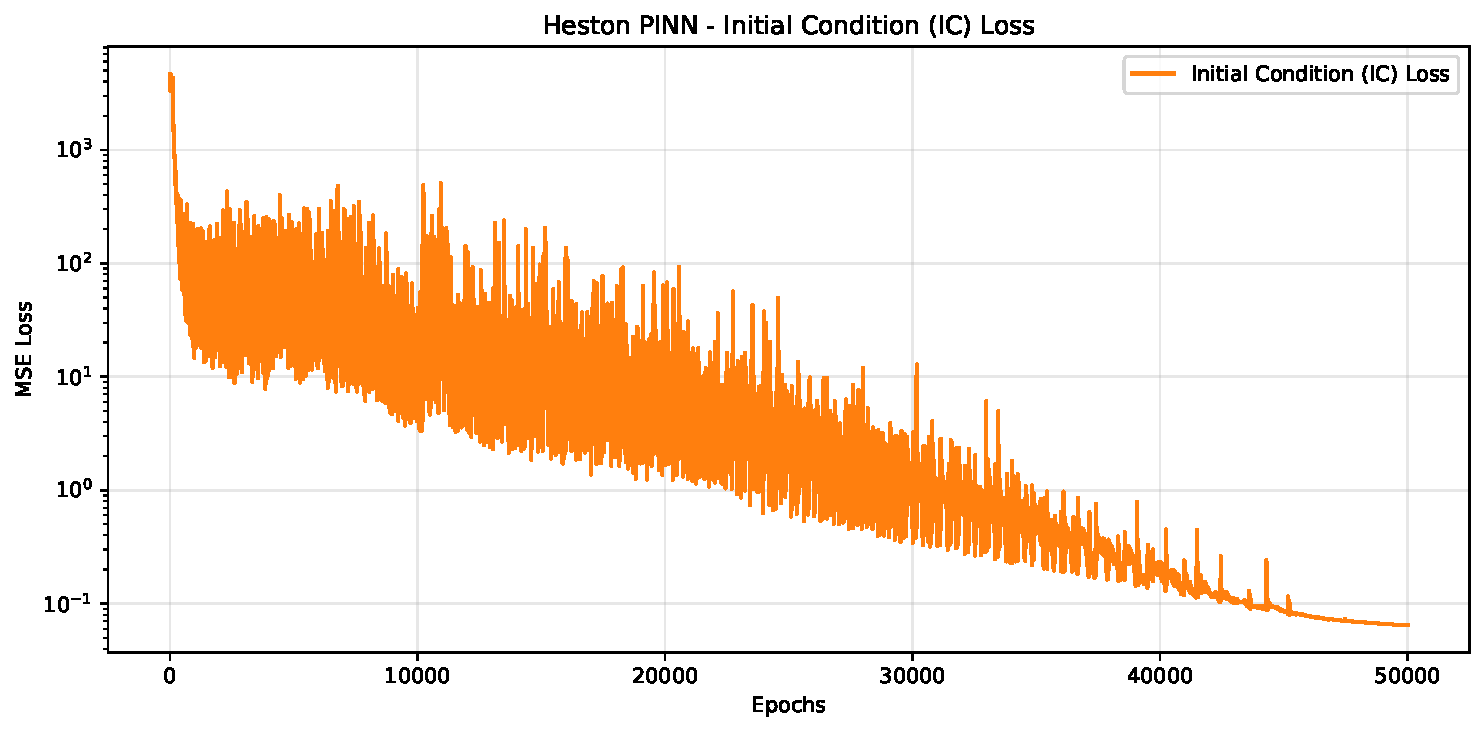
\includegraphics[width=\linewidth]{figures/pinn_hs_loss_ic.pdf}
        \caption{Initial-condition loss for the Heston PINN. This measures how accurately the terminal payoff condition is enforced.}
        \label{fig:pinn_hs_loss_ic.pdf}
    \end{subfigure}
    \hfill
    \begin{subfigure}[t]{0.49\linewidth}
        \centering
        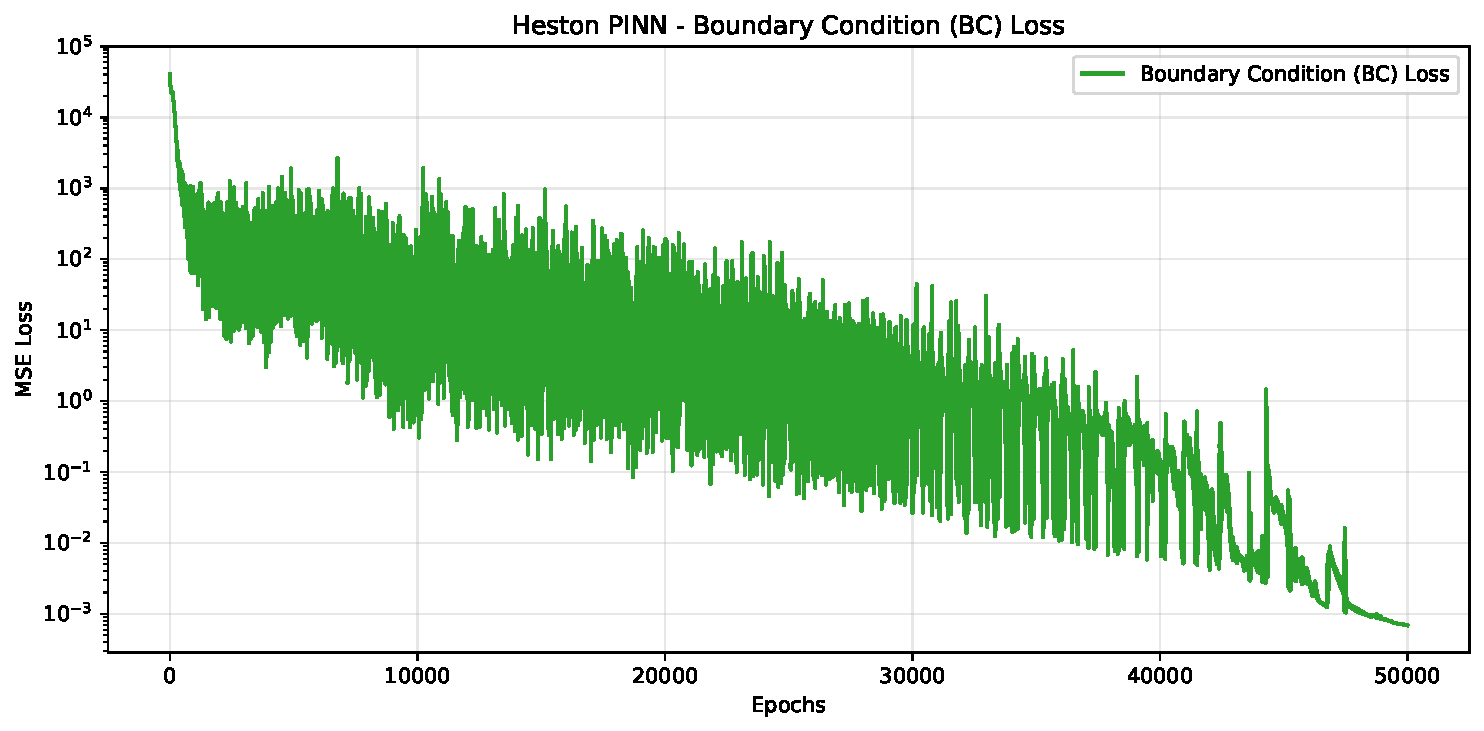
\includegraphics[width=\linewidth]{figures/pinn_hs_loss_bc.pdf}
        \caption{Boundary-condition loss for the Heston PINN. This component shows how well the model respects the imposed boundary behavior during training.}
        \label{fig:pinn_hs_loss_bc.pdf}
    \end{subfigure}

    \caption{Loss decomposition for the final Heston PINN. The four panels show the evolution of the total, PDE, initial-condition, and boundary-condition losses, providing a compact overview of convergence behavior across the full training run.}
    \label{fig:pinn_hs_loss_panel}
\end{figure}


%%%%%%%%%%%%%%%%%%%%%%%%%%%%%%%%%%%%%%%%%%%%%%%%%%%%%%%%%%%%%%%%%%%%%%%%%%%%
%%%%%%%%%%%%%%%%%%%%%%%%%%%%%%%%%%%%%%%%%%%%%%%%%%%%%%%%%%%%%%%%%%%%%%%%%%%%
%%%%%%%%%%%%%%%%%%%%%%%%%%%%%%%%%%%%%%%%%%%%%%%%%%%%%%%%%%%%%%%%%%%%%%%%%%%%


\clearpage\subsection{Inverse PINN}

\begin{figure}[H]
    \centering

    \begin{subfigure}[t]{0.8\linewidth}
        \centering
        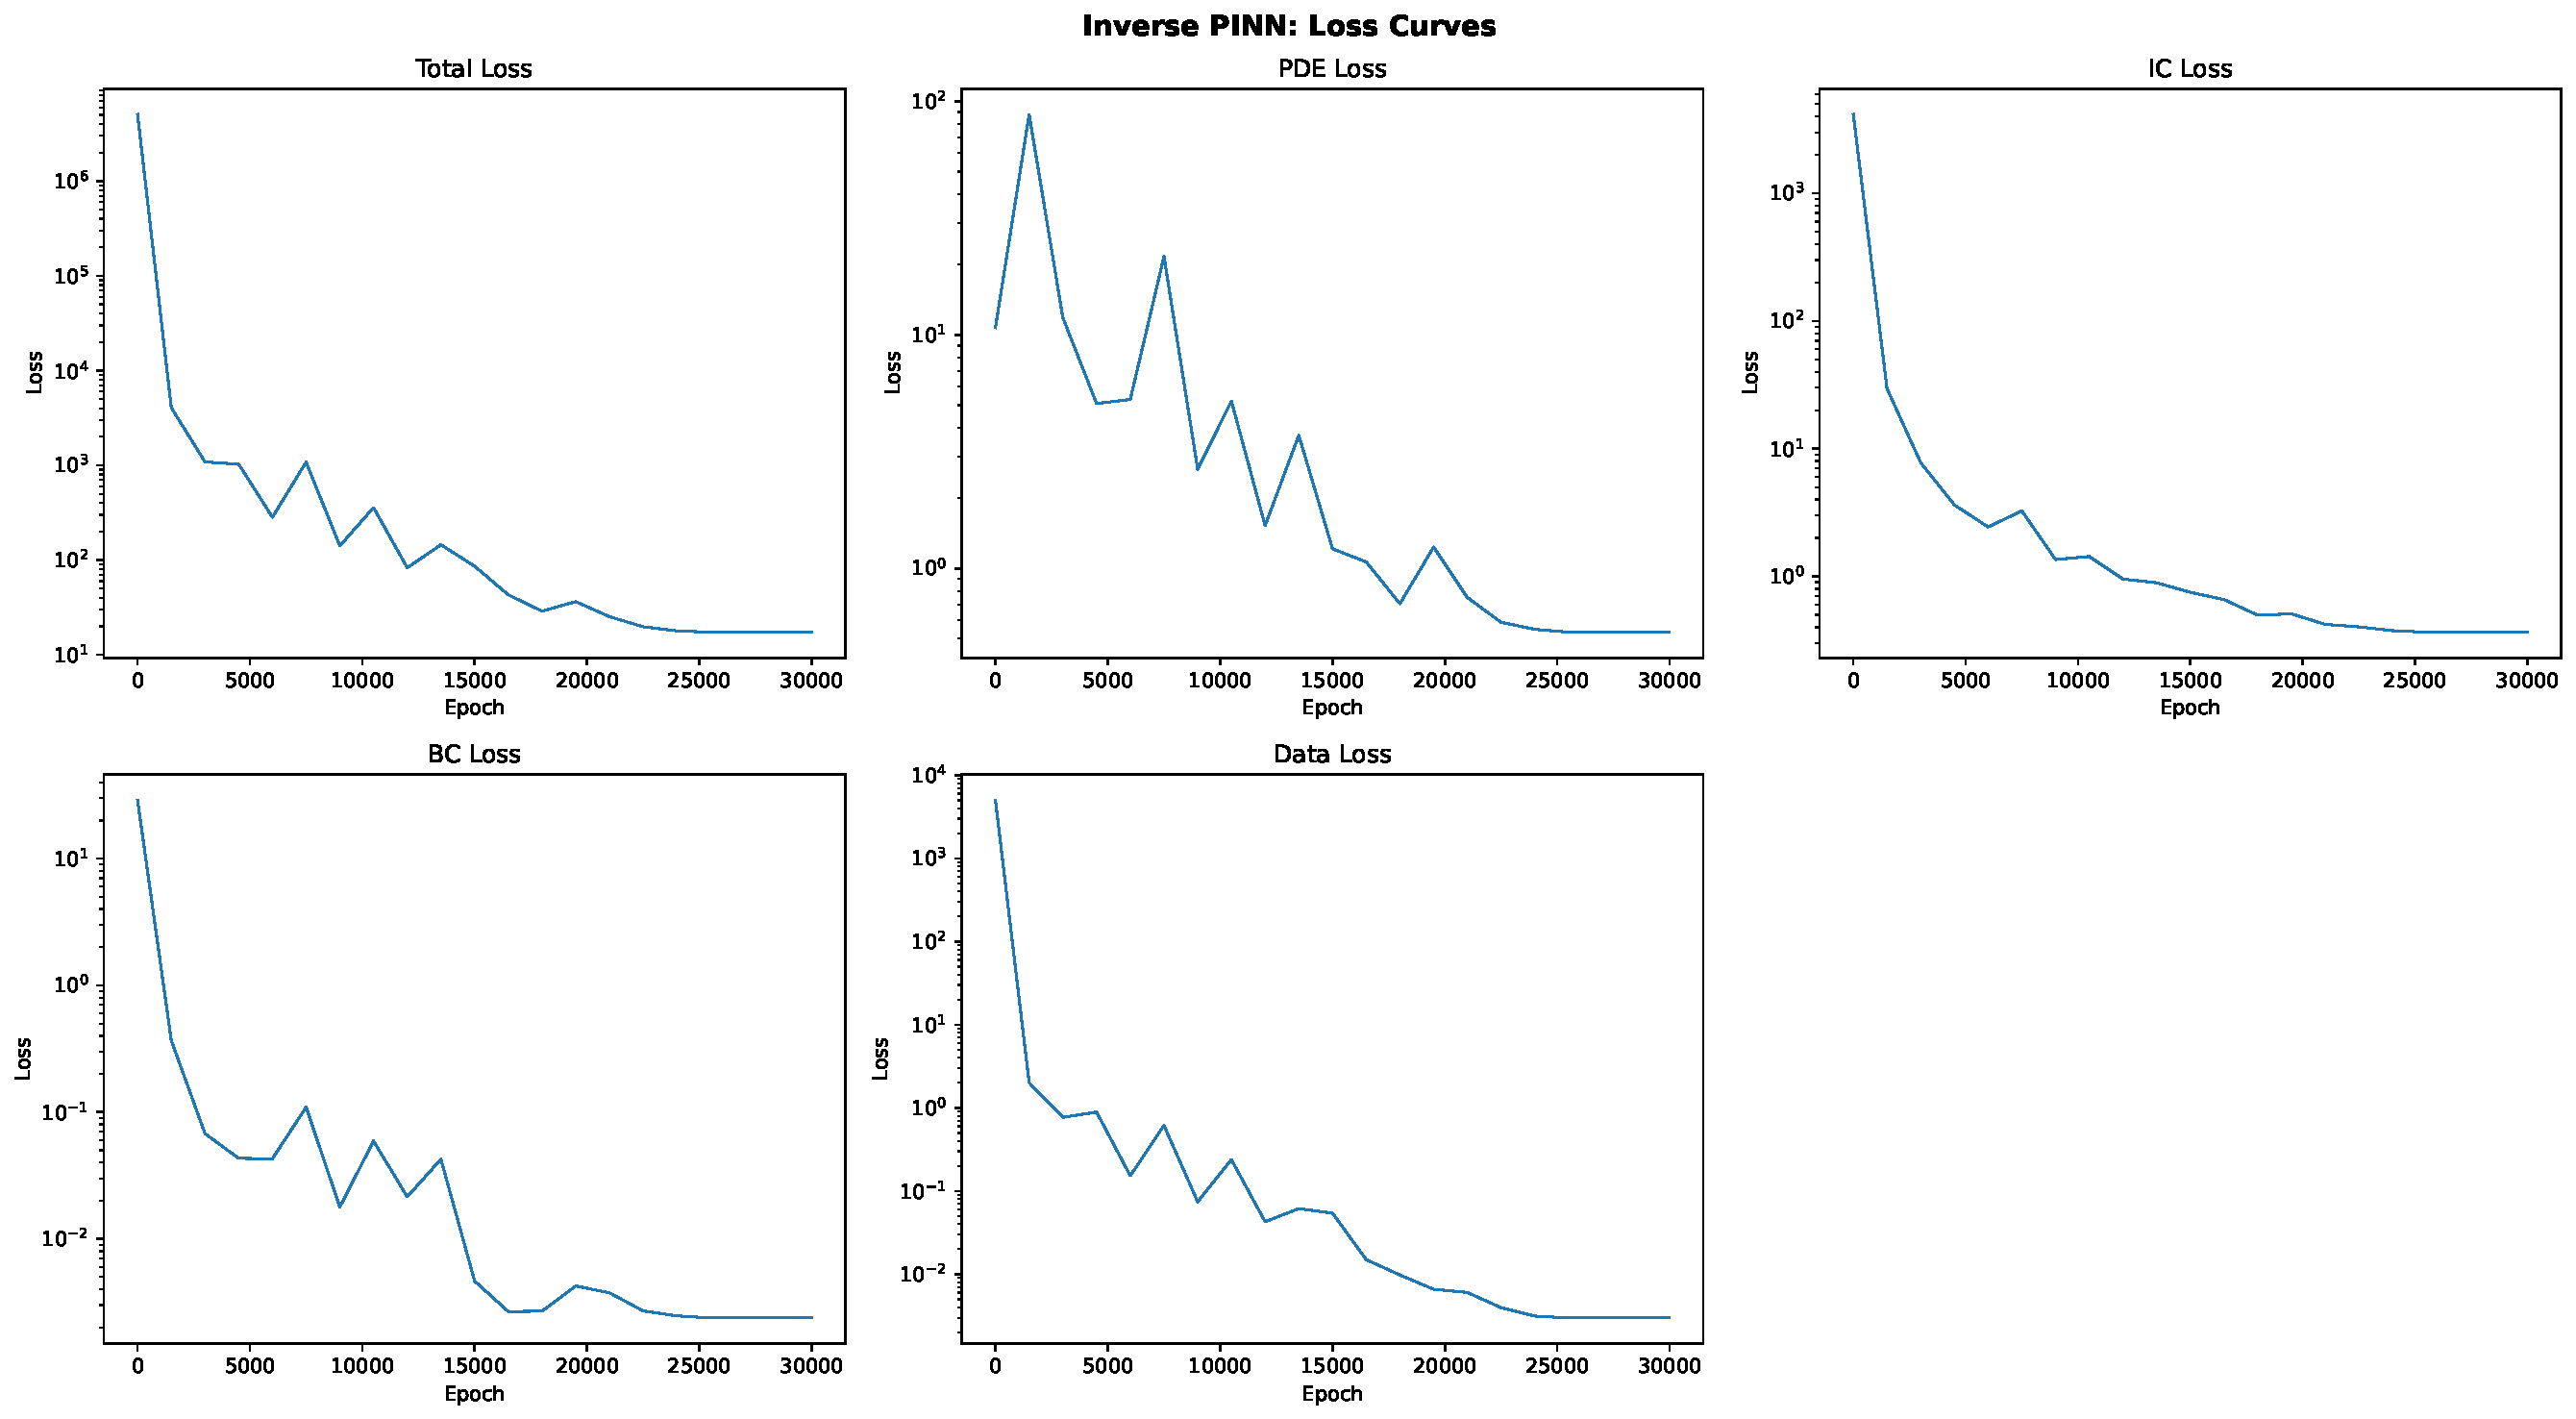
\includegraphics[width=\linewidth]{figures/pinn_inv_losses.pdf}
        \caption{Loss decomposition for the inverse PINN calibration. The figure tracks the optimization objective and its constituent terms, showing how the model balances PDE consistency, boundary and initial conditions, market-data fit, and regularization during training.}
        \label{fig:pinn_inv_losses.pdf}
    \end{subfigure}

    \vspace{0.55cm}

    \begin{subfigure}[t]{0.8\linewidth}
        \centering
        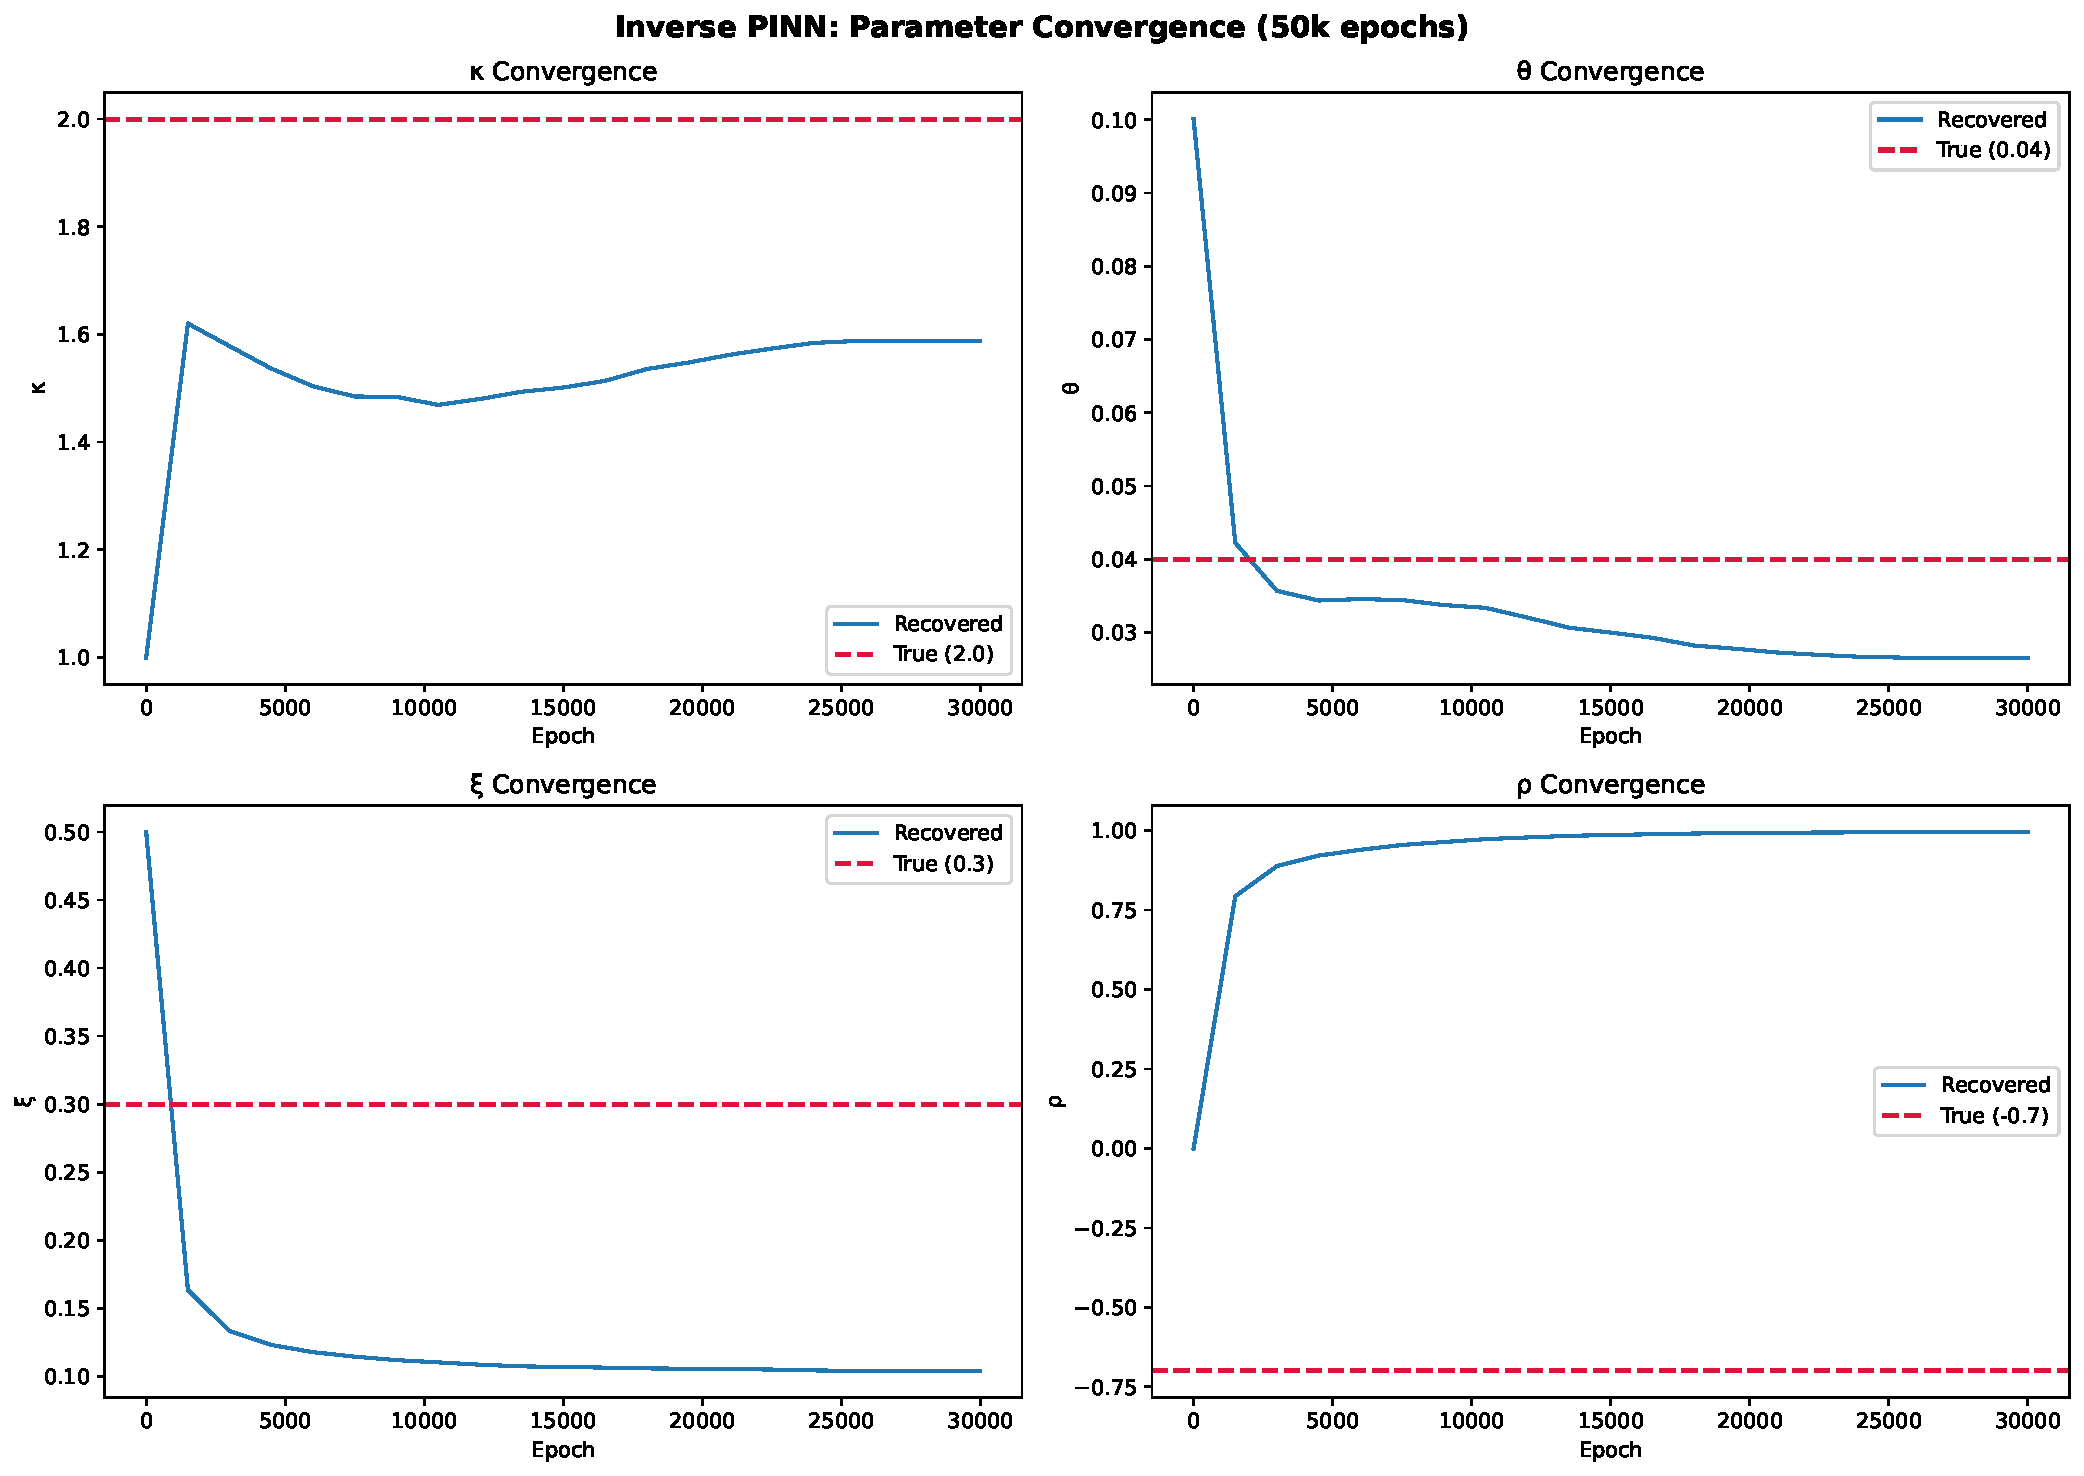
\includegraphics[width=\linewidth]{figures/pinn_inv_params.pdf}
        \caption{Estimated Heston parameters during inverse PINN calibration. The figure shows the evolution of $\kappa$, $\theta$, $\xi$, and $\rho$, giving a direct view of parameter convergence and stability across epochs.}
        \label{fig:pinn_inv_params.pdf}
    \end{subfigure}

    \caption{Inverse PINN calibration diagnostics. The upper panel summarizes loss convergence, while the lower panel shows the corresponding evolution of the calibrated Heston parameters.}
    \label{fig:pinn_inv_diagnostics_panel}
\end{figure}

%%%%%%%%%%%%%%%%%%%%%%%%%%%%%%%%%%%%%%%%%%%%%%%%%%%%%%%%%%%%%%%%%%%%%%%%%%%%
%%%%%%%%%%%%%%%%%%%%%%%%%%%%%%%%%%%%%%%%%%%%%%%%%%%%%%%%%%%%%%%%%%%%%%%%%%%%
%%%%%%%%%%%%%%%%%%%%%%%%%%%%%%%%%%%%%%%%%%%%%%%%%%%%%%%%%%%%%%%%%%%%%%%%%%%%

\begin{figure}[H]
    \centering
    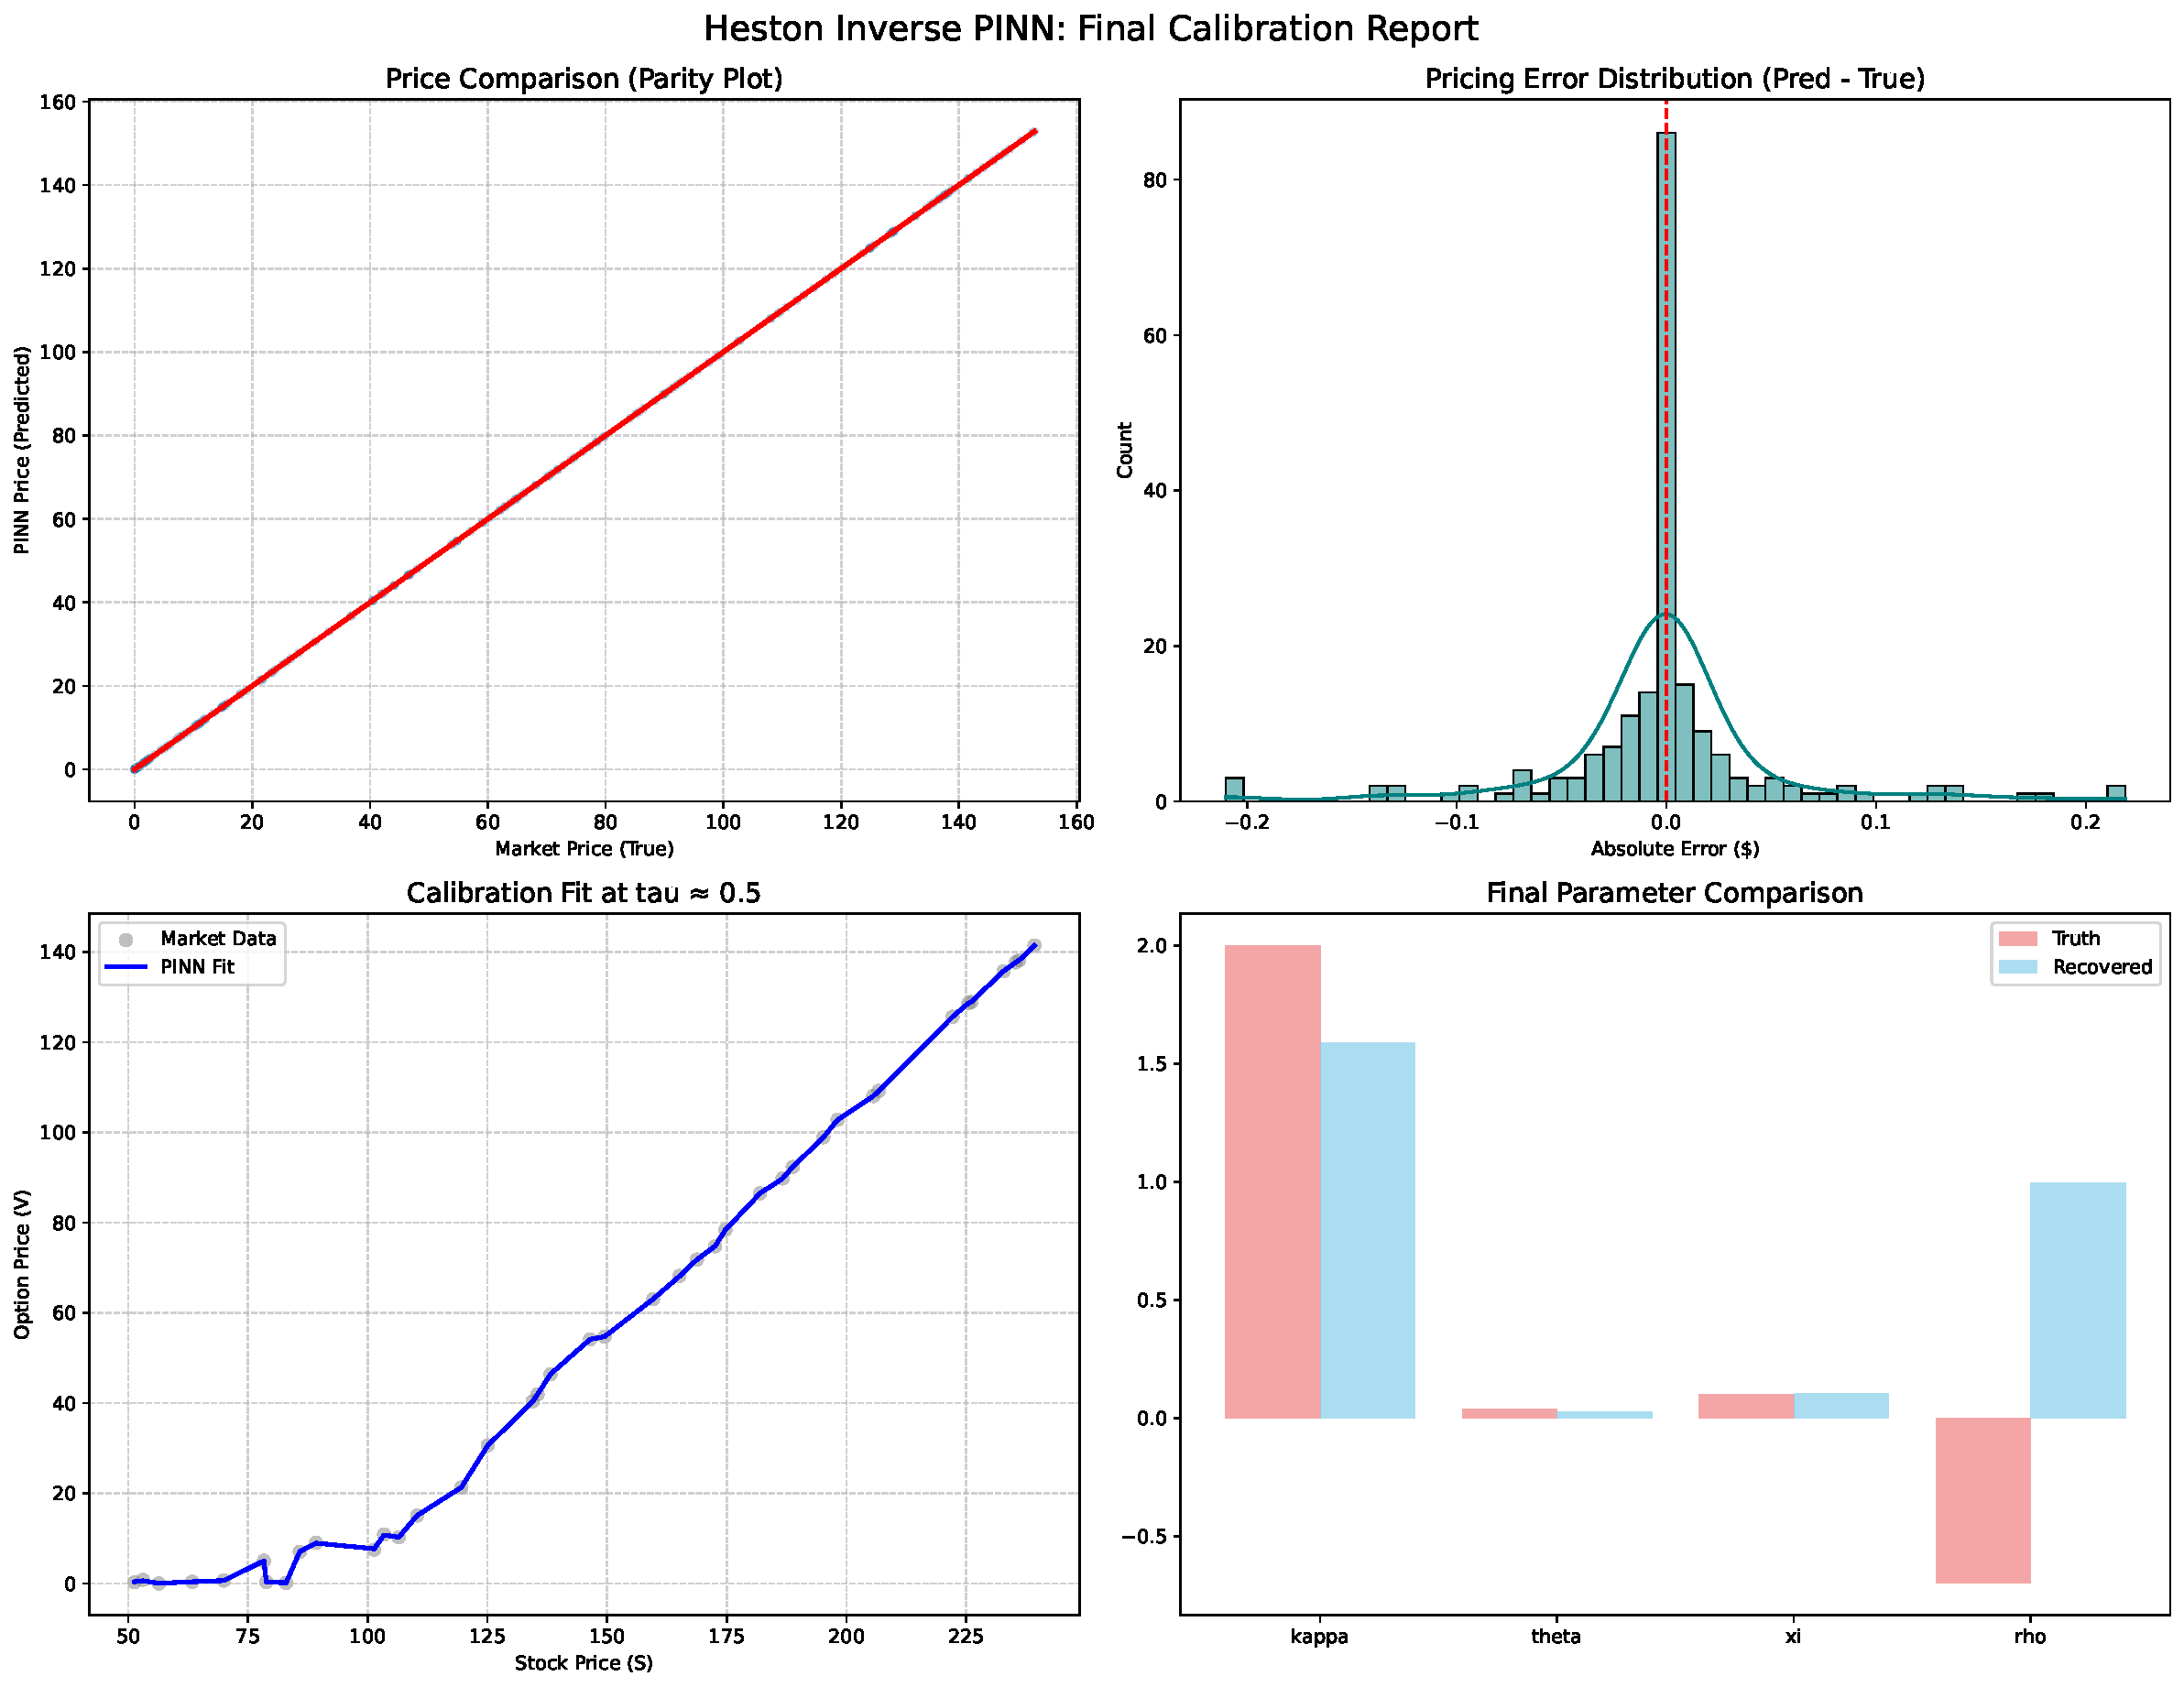
\includegraphics[width=\linewidth]{figures/pinn_inv_final_calibration_report.pdf}
    \caption{Caption}
    \label{fig:placeholder}
\end{figure}

%%%%%%%%%%%%%%%%%%%%%%%%%%%%%%%%%%%%%%%%%%%%%%%%%%%%%%%%%%%%%%%%%%%%%%%%%%%%
%%%%%%%%%%%%%%%%%%%%%%%%%%%%%%%%%%%%%%%%%%%%%%%%%%%%%%%%%%%%%%%%%%%%%%%%%%%%
%%%%%%%%%%%%%%%%%%%%%%%%%%%%%%%%%%%%%%%%%%%%%%%%%%%%%%%%%%%%%%%%%%%%%%%%%%%%